%%%%%%%%%%%%%%%%%%%%%%%%%%%%%%%%%%%%%%%%%%%%%%%%%%%
%
%  New template code for TAMU Theses and Dissertations starting Fall 2012.  
%  For more info about this template or the 
%  TAMU LaTeX User's Group, see http://www.howdy.me/.
%
%  Author: Wendy Lynn Turner 
%	 Version 1.0 
%  Last updated 8/5/2012
%
%%%%%%%%%%%%%%%%%%%%%%%%%%%%%%%%%%%%%%%%%%%%%%%%%%%

%%%%%%%%%%%%%%%%%%%%%%%%%%%%%%%%%%%%%%%%%%%%%%%%%%%%%%%%%%%%%%%%%%%%%%%
%%%                           SECTION V
%%%%%%%%%%%%%%%%%%%%%%%%%%%%%%%%%%%%%%%%%%%%%%%%%%%%%%%%%%%%%%%%%%%%%%
\chapter{\uppercase {Application of the entropy viscosity method to the $1$-D grey radiation-hydrodynamic equations}}\label{chap:hydro}
%%%%%%%%%%%%%%%%%%%%%%%%%%%%%%%%%%%%%%%%%%%%%%%%%%%%%%%%%%%%%
%%%%%%%%%%%%%%%%%%%%%%%%%%%%%%%%%%%%%%%%%%%%%%%%%%%%%%%%%%%%%
\section{Backgrounds}\label{sec:back_sect5}
%%%%%%%%%%%%%%%%%%%%%%%%%%%%%%%%%%%%%%%%%%%%%%%%%%%%%%%%%%%%%
%%%%%%%%%%%%%%%%%%%%%%%%%%%%%%%%%%%%%%%%%%%%%%%%%%%%%%%%%%%%%
Solving the radiation hydrodynamic equations is a challenging task for multiple reasons. First, the characteristic time scales between the radiation and hydrodynamics are different by several orders of magnitude which often requires the radiation part to be solved implicitly to ensure stability. Second, as with any wave-dominated problems, high resolution schemes are needed to accurately resolve shocks. Third, achieving high-order accuracy is challenging but some recent developments provided high-order accuracy results both in time and space when discretizing either the Euler equations \cite{Hussaini, jlg1, jlg2, Leveque} or the radiation equation independently from each other. 

Significant effort has been put into developing Riemann solvers for both the radiation and hydrodynamic equations. Balsara \cite{Balsara} developed a Riemann solver for the radiation-hydrodynamic equations by considering the frozen approximation that decouples the two physics components. However, such an approach may be questionable in the equilibrium diffusion limit. In this case, the coupling terms drive the physics and have to be accounted for. A \emph{generalized Riemann solver} that accounts exactly for the relaxation terms was developed in \cite{Balsara}. Another approach assumes the strong equilibrium diffusion limit in which radiation diffusion is negligible and the radiation simply advects at the material velocity \cite{Woodward}. In this limit, the radiation hydrodynamics equation can be expressed in the form of the Euler equations with a radiation-modified equation of state (REOS) . Any solution technique for the Euler equations may be applied to these equations. Thus, one may develop approximate Riemann solvers for these equations and applied them in a general context. 

Edwards and al. \cite{EdwardsMorelLowrie} proposed a two-stage semi-implicit IMEX scheme to solve the coupled radiation-hydrodynamic equations. They applied a Trapezoidal/BDF2 temporal discretization scheme to the nonlinear grey radiation diffusion. The radiation and hydrodynamic equations are solved implicitly and explicitly, respectively. A Riemann solver along with a flux limiter is used to resolve shocks and other waves. Their results show good agreement with semi-analytical solutions. 

In this section we propose to solve the 1-D radiation-hydrodynamics equations by using \emph{the entropy viscosity method}. The methodology proposed in \sect{sec:hyp_sect1b} will be applied.
%This technique, developed by Guermond et al.  for hyperbolic systems of equations \cite{jlg1, jlg2}, consists in adding appropriate dissipative terms to the governing equations.  The viscosity coefficient of these terms is modulated by the local entropy production. These dissipative terms are devised to stabilize the numerical scheme and to remove the non-physical oscillations appearing at the shock locations. Generally speaking, entropy is produced at shocks \cite{Toro}. Thus, by setting the viscosity coefficient proportional to the entropy production, shocks can be detected and tracked and an adequate amount of viscosity is added locally to stabilize the numerical scheme. The entropy production is computed on the fly, by analyzing the entropy residual. This residual is strongly peaked in shocks and small elsewhere. 
%The entropy viscosity method was shown to achieve high-order accuracy away from the shock regions, was successfully applied to non-linear hyperbolic equations using various discretization methods (finite volume, continuous and discontinuous finite elements, spectral method) and yielded high-order accuracy on non-uniform meshes and complex geometries \cite{jlg2, valentin}. 
Because of the similarity between Euler equations and the radiation hydrodynamic equations, it is conjectured that the entropy viscosity method may be a good candidate for resolving shocks occurring in radiation-hydrodynamic phenomena.

The 1-D grey radiation-hydrodynamic (GRH) equations are recalled in \eqt{eq:equation1}:
\begin{equation}
\label{eq:equation1}
\left\{
\begin{array}{lll}
\partial_t \left( \rho \right) + \partial_x\left( \rho u \right) = 0 \\
\partial_t \left( \rho u\right) + \partial_x \left(\rho u^2 + P + \frac{\epsilon}{3} \right) = 0 \\
\partial_t \left( \rho E\right) + \partial_x \left[ u \left( \rho E + P \right) \right] = -\frac{u}{3} \partial_x \epsilon - \sigma_a c \left( a T^4 - \epsilon \right) \\
\partial_t \epsilon + \frac{4}{3} \partial_x \left( u \epsilon \right) = \frac{u}{3} \partial_x \epsilon + \partial_x \left( \frac{c}{3 \sigma_t} \partial_x \epsilon \right) + \sigma_a c \left( a T^4 - \epsilon \right)
\end{array}
\right. ,
\end{equation}
where $\rho$, $u$, $E$, $\epsilon$, $P$ and $T$ are the material density, material velocity, material specific total energy, radiation energy density, material pressure and temperature, respectively. The total and absorption cross sections, $\sigma_t$ and $\sigma_a$, are either constant or density- and temperature-dependent. The variables $a$ and $c$ are the Boltzman constant and the speed of light, respectively. Lastly, the symbols $\partial_t$ and $\partial_x$ denote the temporal and spatial partial derivatives, respectively. 
The material temperature and pressure are computed with the Ideal Gas equation of state (IGEOS):
\begin{equation}
\label{eq:equation2}
\left\{
\begin{array}{ll}
P = (\gamma-1) C_v \rho T \\
e = C_v T 
\end{array}
\right. ,
\end{equation}
where $e$ is the specific internal energy and is obtained from the expression $e = E - 0.5 u^2$. The heat capacity $C_v$ and the heat ratio coefficient $\gamma$ are assumed constant. 

The objective of this paper is to extend the entropy-based viscosity method to the 1-D grey radiation-hydrodynamic equations. The approach followed in this paper is similar to those of \cite{Balsara, LowrieMorel}: an infinite opacity is assumed and the relaxation terms are ignored in order to make \eqt{eq:equation1} hyperbolic. Then, an entropy equation is derived and used to obtain the functional forms of the viscous stabilization terms. Definitions for the viscosity coefficients are provided. 

This section is organized as follows. In \sect{sec:entropy-visc-meth_sct5}, the entropy viscosity method is extended to the grey radiation-hydrodynamic equations;  details regarding the derivation of the adequate dissipative terms and definitions for the new viscosity coefficients are provided. Numerical results are presented in \sect{sec:num-res} where the second-order accuracy of the scheme is demonstrated in both the equilibrium diffusion and streaming limits, using the method of manufactured solutions applied to the GRH equations. Then, several numerical test cases, taken from the published literature, are provided; in these simulations, the Mach number varies from $1.05$ to $50$ \cite{LowrieEdwards}.

%%%%%%%%%%%%%%%%%%%%%%%%%%%%%%%%%%%%%%%%%%%%%%%%%%%%%%%%%%%%%
%%%%%%%%%%%%%%%%%%%%%%%%%%%%%%%%%%%%%%%%%%%%%%%%%%%%%%%%%%%%%
\section{The Entropy Viscosity Method applied to the 1-D radiation-hydrodynamic equations}\label{sec:entropy-visc-meth_sct5}
%%%%%%%%%%%%%%%%%%%%%%%%%%%%%%%%%%%%%%%%%%%%%%%%%%%%%%%%%%%%%
%%%%%%%%%%%%%%%%%%%%%%%%%%%%%%%%%%%%%%%%%%%%%%%%%%%%%%%%%%%%%

In this section, we extend the entropy viscosity method \cite{jlg1, jlg2, valentin} to the 1-D radiation-hydrodynamic equations in a staged process. First, the reader is guided through the main steps that lead to the derivation of the dissipative terms, using the entropy minimum principle \cite{entropy}. Then, a definition for the entropy viscosity coefficient based upon the entropy production is given. 

\noindent
We recall that the entropy viscosity method was developed for hyperbolic system of equations. However, the radiation hydrodynamic equations are not strictly hyperbolic but several numerical techniques are based on the study of their hyperbolic parts \cite{Balsara, LowrieMorel}. Thus, following the same rationale, the system of equations given in \eqt{eq:equation1} is made hyperbolic by assuming an infinite opacity (the frozen approximation) and by ignoring the relaxation terms. These two assumptions yield the following system of equations:
\begin{equation}
\label{eq:equation3}
\left\{
\begin{array}{lll}
\partial_t \left( \rho \right) + \partial_x\left( \rho u \right) = 0 \\
\partial_t \left( \rho u\right) + \partial_x \left(\rho u^2 + P + \frac{\epsilon}{3} \right) = 0 \\
\partial_t \left( \rho E\right) + \partial_x \left[ u \left( \rho E + P \right) \right] = -\frac{u}{3} \partial_x \epsilon\\
\partial_t \epsilon + \frac{4}{3} \partial_x \left( u \epsilon \right) = \frac{u}{3} \partial_x \epsilon
\end{array}
\right. .
\end{equation}
The jacobian matrix of the hyperbolic terms can be computed to derive the eigenvalues:
\begin{equation}
\label{eq:equation4}
\lambda_1 = u-c_m \text{, } \lambda_{2,3} = u \text{ and } \lambda_4 = u+c_m ,
\end{equation}
where $c_m$ is the radiation-modified material speed of sound and is defined as follows:
\begin{equation}
\label{eq:equation5}
c_m^2 = \underbrace{P_{\rho} + \frac{P}{\rho^2}P_e}_{c_{Euler}^2} + \frac{4 \epsilon}{9\rho}
\end{equation}
with $P_x$ the standard shorthand notation for $\partial_x P$, and $c^2_{Euler}$ denotes the definition of the speed of sound when considering only the 1-D Euler equations.
The above hyperbolic system of equations can be recast in a conservative form. This allows us to assume the existence of an entropy function $s$ \cite{Lax} that depends upon the internal energy $e$, the density $\rho$, and the radiation energy density $\epsilon$. Following some algebra given in \app{app:appendixA}, an equation satisfied by the entropy $s$ is obtained:
\begin{equation}
\label{eq:equation6}
\rho \frac{Ds}{Dt} = \rho \left( \partial_t s + u \partial_x s \right) = 0 \text{, }
\end{equation}
where $\frac{D \cdot}{Dt}$ denotes the total or material derivative. \eqt{eq:equation6} is referred to as the entropy residual and is used to prove the entropy minimum principle, $\frac{Ds}{Dt} \geq 0$, \cite{entropy}.

When adding dissipative terms to each equation of \eqt{eq:equation3} as required in the entropy viscosity method, the entropy residual equation is modified and some additional terms will appear in the right-hand side of \eqt{eq:equation6}. The sign of these extra terms needs to be studied for the entropy minimum principle to hold. As such, the entropy minimum principle is invoked to guide in the derivation of appropriate expressions for each of the dissipative terms. Obtaining the final expression of the dissipative terms is a lengthy process and only the final result along with the key assumptions are stated here. The reader is referred to \app{app:appendixA} for the details of the derivation. The system of equations with the dissipative terms is as follows:
\begin{equation}
\label{eq:equation7}
\left\{
\begin{array}{lll}
\partial_t \left( \rho \right) + \partial_x\left( \rho u \right) = \partial_x \left( \kappa \partial_x \rho \right) \\
\partial_t \left( \rho u\right) + \partial_x \left(\rho u^2 + P + \frac{\epsilon}{3} \right) = \partial_x \left( \kappa \partial_x \rho u \right) \\
\partial_t \left( \rho E\right) + \partial_x \left[ u \left( \rho E + P \right) \right] + \frac{u}{3} \partial_x \epsilon = \partial_x \left( \kappa \partial_x(\rho E) \right)\\
\partial_t \epsilon + \frac{4}{3} \partial_x \left( u \epsilon \right) - \frac{u}{3} \partial_x \epsilon = \partial_x \left( \kappa \partial_x \epsilon \right)
\end{array}
\right. ,
\end{equation}
where $\kappa$ is a locally defined positive viscosity coefficient. It was assumed the following conditions hold:
\begin{equation}
\label{eq:equation7bis}
\left\{
\begin{array}{ll}
P \frac{\partial s}{\partial e} + \rho^2 \frac{\partial s}{\partial \rho} + \frac{4}{3} \rho \epsilon \frac{\partial s}{\partial \epsilon} = 0 \\
s( \rho, e, \epsilon) = \hat{s}(\rho, e) + \frac{\rho_0}{\rho}\tilde{s}(\epsilon) 
\end{array}
\right.
\end{equation}
where $\tilde{s}$ is concave with respect to the radiation energy density $\epsilon$ and $\hat{s}$ is concave with respect to the internal energy $e$ and the specific volume $\rho^{-1}$. The constant $\rho_0$ is of order one and appears only for dimensionality purposes. The function $\hat{s}$ and $\tilde{s}$ are both physical entropy functions.

Once the dissipative terms are obtained, it remains to define the local viscosity coefficient $\kappa(x,t)$. Note that at the difference of the multi-D Euler equations of \sect{chap:euler}, only one viscosity coefficient is required since the low Mach asymptotic limit is not investigated in this section. In other word, it is assumed that $\mu(x,t) = \kappa(x,t)$ following the notations used in \sect{chap:euler}. 
We require the following to hold in the prescription for $\kappa$:
\begin{itemize}
\item Since the entropy residual is a measure of the entropy production that occurs in shock regions, it is natural to define a viscosity coefficient proportional to the entropy residual. This will enable shock detection and tracking and will also provide a measure of the viscosity required to stabilize the scheme. This viscosity coefficient is referred to as the \emph{entropy viscosity coefficient} or \emph{second-order viscosity coefficient} and is denoted by $\kappa_e(x,t)$.
\item An upper bound on $\kappa$ is to be set since entropy production can be very large in shocks. For explicit time integration, the maximum value of the viscosity coefficient is related to the Courant-Friedrichs-Lewy number (CFL). The upper bound on  $\kappa$  is defined by analogy to the standard upwind (Godunov) scheme that is known to efficiently smooth out oscillations (but is only first-order accurate). With implicit temporal integrators, the same reasoning is used even if the CFL number may not need to be strictly respected. This upper bound will be referred to as the \emph{first-order viscosity}, denoted by $\kappa_{max}(x,t)$.  
\item The viscosity coefficient $\kappa$ that is actually used in the dissipative terms of \eqt{eq:equation3} is defined as follows: $\kappa(x,t) = \min ( \kappa_e(x,t), \kappa_{max}(x,t) )$. With such a definition, the viscosity added to the system of equations will saturate to the first order viscosity in the shock regions. Elsewhere, the entropy production and thus the viscosity coefficient $\kappa$ are expected to be small.
\end{itemize}

Next, we define the local first- and second-order viscosity coefficients $\kappa_{max}(x,t)$ and $\kappa_e(x,t)$, respectively. Following the work of Zingan et al. \cite{valentin}, the first-order viscosity definition is based on the local largest eigenvalue that is known to be $|u| + c_m$ in 1-D:
\begin{equation}
\label{eq:equation8}
\kappa_{max} = \frac{h}{2} \left( |u| + c_m \right)
\end{equation}  
where $h$ is the local grid size. This definition is derived based on the upwind scheme and a simple derivation can be found in \cite{jlg1} in the case of a scalar hyperbolic equation. Through the definition of the radiation-modified speed of sound $c_m$, both the material and radiation properties are accounted for in the definition of the first-order viscosity coefficient.

\noindent 
The definition of the second order viscosity coefficient $\kappa_e(x,t)$ is based upon the entropy residual (\eqt{eq:equation6}) recast as a function of pressure $P$, density $\rho$ and radiation energy density $\epsilon$:
\begin{equation}
\label{eq:equation9}
R(x,t) = \frac{s_e}{P_e} \underbrace{ \left( \frac{dP}{dt} - c_{Euler}^2 \frac{d\rho}{dt} \right)}_\textrm{$\hat{R}(x,t)$}
\end{equation}
The term $s_e$ is the inverse of the material temperature (\app{app:appendixA}) and $P_e$ is computed from the IGEOS. These two terms are positive so that the sign of the entropy residual $R(x,t)$ can be determined by simply inspecting the terms inside the parentheses, denoted by $\hat{R}(x,t)$. Such an expression is easier to compute than the one given in \eqt{eq:equation6} which required an analytical expression for the entropy function. In addition to the entropy residual, inter-element jumps in the pressure and density gradients, $J$, are also accounted for. The objective is to be able to also detect discontinuities that are not shocks, such as contact waves (there is no entropy production in a contact wave), in order to stabilize them as well. 

Thus, the entropy viscosity coefficient $\kappa_e(x,t)$ is set to be proportional to $\hat{R}(x,t)$ and $J$ with the following form: 
\begin{equation}
\label{eq:equation12}
\kappa_e(x,t) = h^2 \frac{\max (|\hat{R}(x,t)|, J)}{n_P}
\end{equation} 
where $J = \max_i (J(x_i,t))$, and $J(x_i,t)$ is the jump of a given quantity at cell interface $x_i$, and $n_P$ is a normalization function (of the same units as pressure) that has to be chosen so that the viscosity coefficient $\kappa$ has units of $m^2/s$. The following definition for the normalization function has been chosen: $n_P = \rho c_m^2$. Thus, the final definition for the viscosity coefficient $\kappa$ is the following:
\begin{equation}
\label{eq:equation12bis}
\kappa_e(x,t) = h^2 \frac{\max (|\hat{R}(x,t)|, J)}{\rho c_m^2}
\end{equation} 
The jump $J$ in the definition of $\kappa(x,t)$ is piecewise-constant. Its definition is discretization-dependent and defined as follows for Continuous Galerkin FEM: 
\begin{equation}
\label{eq:equation12ter}
\left\{
\begin{array}{lll}
J_P(x_i,t) = |u| [[\partial_x P]]\\
J_{\rho}(x_i,t) = c_m^2 |u|  [[\partial_x \rho]] \\
J(x_i,t) = \max( J_{\rho}(x_i,t), J_{P}(x_i,t) )
\end{array}
\right.
\end{equation}
The symbol $[[ \cdot ]]$ denotes the jump at the cell interface.

The entropy viscosity method is now well defined for the hyperbolic system given in \eqt{eq:equation3} and will be used to solve for the grey radiation-hydrodynamic equations given in \eqt{eq:equation1}. However, one may question how the relaxation source terms, $\sigma_a c (a T^4-\epsilon)$ and the physical diffusion term, $\partial_x(D\partial_x \epsilon)$, may affect the entropy viscosity method. When applying the entropy viscosity method, the radiation energy density equation will now contain a diffusive term and a numerical dissipative term with a vanishing viscosity coefficient $\kappa$. As long as the diffusive coefficient $D=\frac{c}{3 \sigma_t}$ is larger than the viscosity coefficient $\kappa$, the numerical dissipative term should not be required. A way to ensure consistency and prevent the formation of oscillations in the frozen limit is to merge the two second-order derivative terms into one as follows:
\begin{equation}
 \partial_x \left( \frac{c}{3 \sigma_t} \partial_x \epsilon \right) + \partial_x \left( \kappa \partial_x \epsilon \right) 
 \Longrightarrow
 \partial_x \left[ \max\left(\frac{c}{3 \sigma_t} \text{, } \kappa \right) \partial_x \epsilon \right]
\end{equation}
Thus, as long as the artificial viscosity coefficient $\kappa$ is locally smaller that the physical diffusive coefficient $D=\frac{c}{3 \sigma_t}$, no artificial viscosity is required to ensure stability of the numerical scheme. As the diffusive coefficient $D$ goes to zero, shocks can form in the radiation energy density profile and will require a certain amount of viscosity in order to prevent oscillations from appearing.

The effect of the relaxation source terms onto the entropy viscosity method can become problematic in the equilibrium diffusion limit $(\sigma_a c \to \infty)$: the relaxation source terms behave as dissipative terms and make the system parabolic \cite{Leveque}. In \cite{ShiJin}, a study on the impact of various artificial viscosity methods onto hyperbolic systems with relaxation terms was carried out. It was shown that high-order viscosity coefficients are more suitable since they do not alter the physical solution as much as first-order viscosity terms (upwind scheme). A manufactured  solution is employed in \sect{sec:MMS} to test the convergence of the numerical solution in the equilibrium-diffusion limit.  
%\begin{remark}
The normalization factor has to be larger than $h$ in order to conserve high-order accuracy.
%\end{remark}

 %\begin{remark}
The reader will notice that, except for the definition of the jumps, the whole method is independent of the spatial discretization employed. The technique could be used with discontinuous Galerkin finite element or finite volume methods. In both cases, an adequate  definition of the jump terms can be found in \cite{valentin}.
 %\end{remark}

%%%%%%%%%%%%%%%%%%%%%%%%%%%%%%%%%%%%%%%%%%%%%%%%%%%%%%%%%%%%%
%%%%%%%%%%%%%%%%%%%%%%%%%%%%%%%%%%%%%%%%%%%%%%%%%%%%%%%%%%%%%
\section{Numerical results}
\label{sec:num-res}
%%%%%%%%%%%%%%%%%%%%%%%%%%%%%%%%%%%%%%%%%%%%%%%%%%%%%%%%%%%%%
%%%%%%%%%%%%%%%%%%%%%%%%%%%%%%%%%%%%%%%%%%%%%%%%%%%%%%%%%%%%%

In this section, numerical results using the entropy viscosity method are presented for the dimensional 1-D grey radiation-hydrodynamic equations. First, second-order accuracy of the method is demonstrated using the method of manufactured solution (MMS). Then, results for some standard radiation-hydrodynamic test cases are given. Details of the temporal and spatial discretizations for a the CGFEM employed in the multi physics MOOSE framework \cite{Moose} are given in \sect{sec:disc_sect2}.
%%%%%%%%%%%%%%%%%%%%%%%%%%%%%%%%%%%%%%%%%%%%%%%%%%%%%%%%%%%%%
\subsection{Space/time accuracy}
\label{sec:MMS}
%%%%%%%%%%%%%%%%%%%%%%%%%%%%%%%%%%%%%%%%%%%%%%%%%%%%%%%%%%%%%

The same manufactured solution as in \cite{EdwardsMorelLowrie} is used in order to test both the diffusive and streaming limit solutions in a slab of thickness $L=2 \pi$ $cm$. The manufactured solutions are composed of trigonometric functions. Periodic boundary conditions are used for all of the variables. The L$_2$ norm of the error between the numerical and exact solutions are computed for density, momentum, total material energy, and radiation energy density. \newpage For each new simulation, the time step is divided by two and the  number of spatial degrees of freedom is doubled. With such settings, the error is expected to decrease by a factor $4$ if second-order convergence is achieved.
The first manufactured solution is designed to test the equilibrium-diffusion limit. In that case, the radiation energy is in equilibrium with the material temperature and the opacity is large which means that the radiation mean-free path is not resolved but the variation of the solution is resolved. The following exact solution was used:
\begin{equation}
\label{eq:equation13}
\left\{
\begin{array}{llll}
\rho = \sin (x-t)+2 \\
u = \cos(x-t) +2 \\
T = \frac{0.5 \gamma (\cos(x-t) +2) }{\sin (x-t)+2}\\
\epsilon = a T^4
\end{array}
\right. .
\end{equation}
The cross sections $\sigma_a$ and $\sigma_t$ are assumed constant and set to the same value $1000$ $cm^{-1}$. The simulation is run until $t=3$ $sh$
(1 $sh$ = $10^{-8}$ $sec$). The L$_2$ error norm along with its ratio between consecutive simulations are given in \tbl{tbl:table1} for the equilibrium diffusion limit case.

\begin{table}[h]
\caption{\label{tbl:table1} L$_2$ norms of the error for for the equilibrium diffusion limit case using a manufactured solution.}
\begin{center}
\begin{tabular}{|c|c|c|c|c|c|c|c|c|c|}
\hline
\textbf{\# of cells} & time step size $(sh)$  & $\mathbf{\rho}$ & \textbf{ratio} & $\mathbf{\rho E}$ & \textbf{ratio} \\ \hline
$20$ & $10^{-1}$ &	 $0.590766$ & NA &  $1.333774$ & NA \\ \hline
$40$ & $5$ $10^{-1}$ & $0.290626$ & $2.03$ &  $0.478819$ & $2.79$ \\ \hline
$80$ & $2.5$ $10^{-2}$ & $0.0959801$ & $3.021$ &  $0.154119$ & $3.11$ \\ \hline
$160$ & $1.25$ $10^{-2}$ & $0.02593738$ & $3.70$ &  $0.0405175$ & $3.80$ \\ \hline
$320$ & $6.25$ $10^{-3}$ & $6.471444$ $10^{-3}$ & $4.00$ & $9.90446$ $10^{-3}$ & $4.09$ \\ \hline
$640$ & $3.125$ $10^{-3}$ & $1.584158$ $10^{-3}$ & $4.01$ & $2.44727$ $10^{-3}$ & $4.04$ \\ \hline
\hline
\textbf{\# of cells} & time step size $(sh)$  & $\mathbf{\epsilon}$ & \textbf{ratio} &  $\mathbf{\rho u}$ & \textbf{ratio} \\ \hline
$20$ & $10^{-1}$ &  $0.00650085$ & NA & $0.910998$ & NA	\\ \hline
$40$ & $5$ $10^{-1}$ &  $0.00124983$ & $5.20$ & $0.4090946$ & $2.23$	\\ \hline
$80$ & $2.5$ $10^{-2}$ &  $0.000262797$ & $4.76$ & $0.125943$ & $3.25$	\\ \hline
$160$ & $1.25$ $10^{-2}$ &  $6.17726$ $10^{-5}$ & $4.25$ & $3.381042$ $10^{-3}$ & $3.72$	\\  \hline
$320$ & $6.25$ $10^{-3}$ & $1.509184$ $10^{-5}$ & $4.09$ & $8.373657$ $10^{-3}$ & $4.04$ \\ \hline 
$640$ & $3.125$ $10^{-3}$  & $3.72548$ $10^{-6}$ & $4.05$ & $2.070538$ $10^{-3}$ & $4.04$ \\ \hline   
\end{tabular}  
\end{center}
\end{table}
\newpage

The second manufactured solution is used to test the method in the streaming limit: the radiation streaming dominates the absorption/re-emission term and evolves at a fast time scale. The exact solution used is as follows :
\begin{equation}
\label{eq:equation14}
\left\{
\begin{array}{llll}
\rho = \sin(x-t)+2 \\
u = \left( \sin(x-t)+2 \right)^{-1} \\
T = 0.5 \gamma \\
\epsilon = \sin(x-1000 t)+2
\end{array}
\right.
\end{equation}
For this manufactured solution, the cross sections are still assumed constant and set to the same value $1$ $cm^{-1}$. The final time is $t_{final}=3$ $sh$. Once again, the L$_2$ error norm is given in \tbl{tbl:table2} for the density, momentum, material total energy and radiation energy density.
\begin{table}[h]
\begin{center}
\caption{\label{tbl:table2} L$_2$ norms of the error for for the streaming limit case using a manufactured solution.}
\begin{tabular}{|c|c|c|c|c|c|}
\hline
\textbf{\# of cells} & time step size $(sh)$  & $\mathbf{\rho}$ & \textbf{ratio} & $\mathbf{\rho E}$ & \textbf{ratio} \\ \hline
$20$ &$10^{-1}$& $1.4373$ $10^{-2}$ & NA & $5.88521$ $10^{-1}$ & NA \\ \hline
$40$ & $5.$ $10^{-2}$& $3.760208$ $10^{-3}$ & $3.82$ & $1.4244$ $10^{-1}$ & $4.13$ \\ \hline 
$80$ & $2.5$ $10^{-2}$& $9.91724$ $10^{-4}$ & $3.79$ & $3.2047$ $10^{-2}$ & $4.44$  \\ \hline      
$160$ & $1.25$ $10^{-2}$ & $2.4455$ $10^{-4}$ & $4.06$ & $7.4886$ $10^{-3}$ & $4.28$  \\ \hline     
$320$ & $6.25$ $10^{-3}$ & $6.280715$ $10^{-5}$ & $3.89$ & $1.82327$ $10^{-3}$ & $4.11$ \\ \hline 
$640$ & $3.125$ $10^{-3}$ & $1.57920$ $10^{-5}$ & $3.98$ & $4.50463$ $10^{-4}$ & $4.05$  \\ \hline
$1280$ & $1.5625$ $10^{-4}$ & $3.96096$ $10^{-6}$ & $3.99$ & $1.12061$ $10^{-4}$ & $4.02$ \\ \hline
\hline
\textbf{\# of cells} & time step size $(sh)$  & $\mathbf{\epsilon}$ & \textbf{ratio} &  $\mathbf{\rho u}$ & \textbf{ratio} \\ \hline
$20$ &$10^{-1}$ & $3.82001$ $10^{-1}$ & NA & $2.354671$ $10^{-3}$ & NA \\ \hline
$40$ & $5.$ $10^{-2}$ & $1.21500$ $10^{-1}$ &$3.14$& $6.138814$ $10^{-4}$& $3.84$ \\ \hline
$80$ & $2.5$ $10^{-2}$ & $3.27966$ $10^{-2}$ &$3.70$& $1.74974$ $10^{-4}$ & $3.51$ \\ \hline
$160$ & $1.25$ $10^{-2}$ & $8.38153$ $10^{-3}$ &$3.91$& $3.61297$ $10^{-5}$  & $4.84$ \\ \hline
$320$ & $6.25$ $10^{-3}$ & $2.10925$ $10^{-3}$ &$3.97$& $9.03866$ $10^{-6}$ & $3.99$ \\ \hline
$640$ & $3.125$ $10^{-3}$ & $5.28472$ $10^{-4}$ &$3.99$& $2.25649$ $10^{-6}$ & $4.01$ \\ \hline
$1280$ & $1.5625$ $10^{-4}$ &$1.322268$ $10^{-4}$ &$3.99$& $5.69984$ $10^{-7}$ & $3.95$ \\ \hline
\end{tabular}
\end{center}
\end{table}
For both manufactured solutions the error is divided by four as the time step and the spatial mesh are reduced by a factor two. Thus, we conclude that GRH equations can be numerically solved with second-order accuracy using the entropy viscosity method when the exact solution is smooth. 

%%%%%%%%%%%%%%%%%%%%%%%%%%%%%%%%%%%%%%%%%%%%%%%%%%%%%%%%%%%%%
\subsection{Radiation shock simulations}
\label{sec:simulations}
%%%%%%%%%%%%%%%%%%%%%%%%%%%%%%%%%%%%%%%%%%%%%%%%%%%%%%%%%%%%%

The purpose of this section is to show that the entropy-based viscosity method (\sect{sec:entropy-visc-meth_sct5}) can accurately resolve shocks occurring in radiation-hydrodynamic simulations. Multiple test cases are considered, with Mach numbers of $1.05$, $1.2$, $2$, $5$ and $50$ \cite{LowrieEdwards}. All of the simulations are run with $500$ spatial cells and with a Courant-Friedrichs-Lewy (CFL number) of $10$ until steady-state (even if the scheme employed here is fully implicit, a CFL number can still be computed and is a good reference for comparison against semi-implicit or fully explicit codes). Linear Lagrange polynomials and the second-order temporal integrator BDF2 are once again used. For clarity, the initial conditions for each test case will be recalled in a table and plots of the density, $\rho (x)$, the radiation temperature, $\theta (x)$, and material temperature, $T(x)$,  at steady-state will be given as well as those of the viscosity coefficients, $\kappa(x)$ and $\kappa_{max}(x)$. The computational domain consists of a 1-D slab of thickness $L$. The initial discontinuity between the left and right states is located at $x_0$ and will be specified for all test cases. For all of the test cases presented in this paper, the cross sections $\sigma_a$ and $\sigma_t$ are assumed constant and set to $853.144$ $cm^{-1}$ and $390.711$ $cm^{-1}$, respectively, if not otherwise specified. The heat capacity at constant specific volume is set to $C_v = 0.12348$ $jerks/(g-keV)$.

For the Mach $2$ simulation, results will also be shown when employing only the first-order viscosity $(\kappa(x,t) = \kappa_{max}(x,t))$ in order to show the benefits of using a high-order viscosity coefficient. 

The inlet and outlet boundary conditions (BCs) are given next. The Euler equations and radiation equation are considered independently since the latter one is parabolic. At the inlet, the flow is supersonic and, therefore, no physical information exits the system. Thus, Dirichlet boundary condition can be used. At the outlet, the flow become subsonic which requires a particular treatment. Following the work from \cite{SEM}, a static boundary condition is implemented. Only the back pressure is provided and the other variables are computed using the characteristic equations. For the radiation equation, vacuum boundary conditions are used at both inlet and outlet.

\newpage
%%%%%%%%%%%%%%%%%%%%%%%%%%%%%%%%%%%%%%%%%%%%%%%%%%%%%%%%%%%%%
\subsubsection{An equilibrium diffusion test}
%%%%%%%%%%%%%%%%%%%%%%%%%%%%%%%%%%%%%%%%%%%%%%%%%%%%%%%%%%%%%

For this test, the inlet Mach number is set to $1.05$. The radiation field and material are in equilibrium. The initial conditions are given in \tbl{tbl:table3}.
\begin{table}[H]
\begin{center}
\caption{\label{tbl:table3} Initial conditions for mach $1.05$.}
\begin{tabular}{|c|c|c|}
\hline 
 & left  & right \\ \hline
$\rho$ $(g/cm^3)$ &$1.$ & $1.0749588$ \\ \hline
$u$ $(cm/sh)$& $0.1228902$ & $0.1144127$ \\ \hline
$T$ $(keV)$& $0.1$ & $0.1049454$\\ \hline
$\epsilon$ $(jerks/cm^3)$ & $1.372$ $10^{-6}$ & $1.6642117$ $10^{-6}$\\
\hline
\end{tabular}
\end{center}  
\end{table}  
The computational domain is of size $L=0.08$ $cm$ and the initial step is at $x_0 = 0.015$ $cm$. The numerical solutions at steady state are given in \fig{fig:Mach105_temp}, \fig{fig:Mach105_density} and \fig{fig:Mach105_viscosity}. 
\begin{figure}[H]
                \centering
                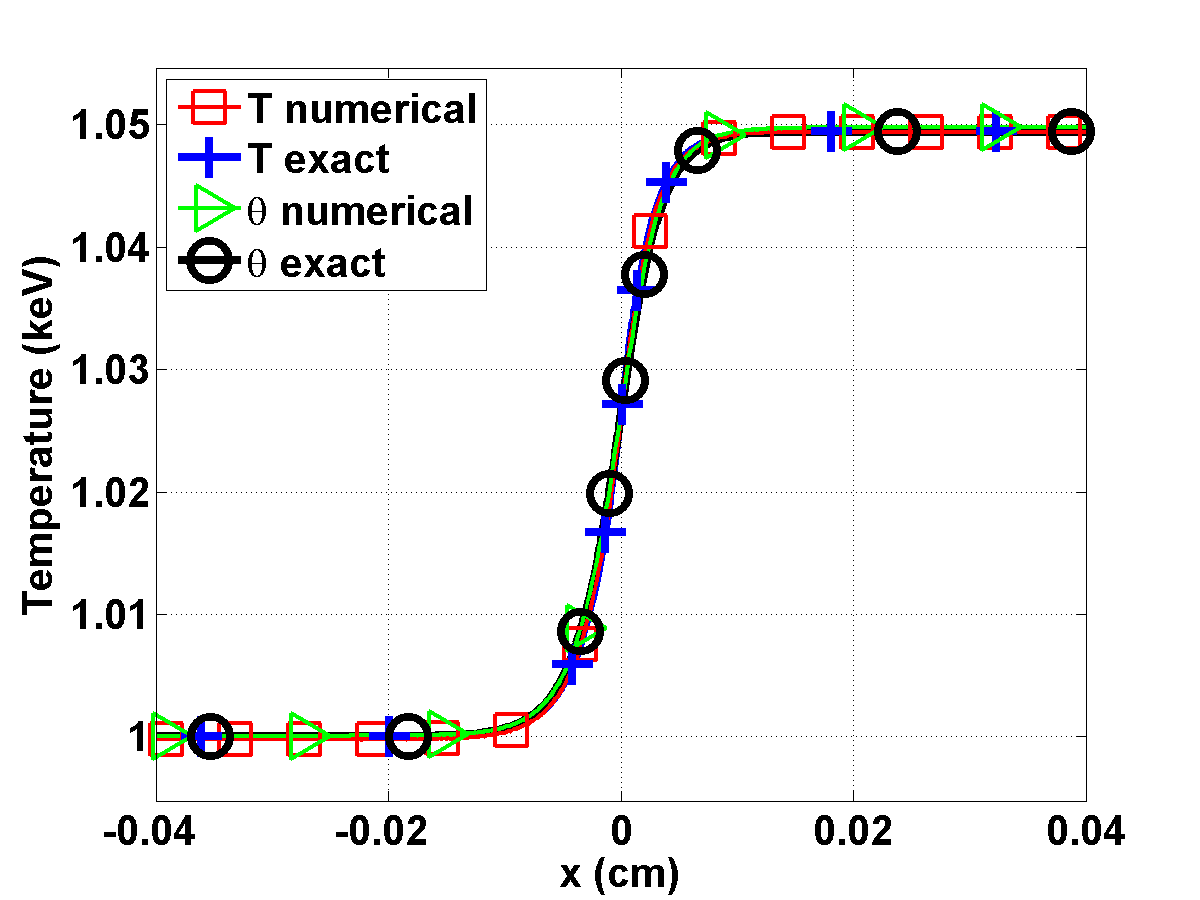
\includegraphics[width=\textwidth]{figures/Mach_1p05_nel_500_temperature.png}
        \caption{Material and radiation temperature profiles at steady state for Mach 1.05 test.}\label{fig:Mach105_temp}
\end{figure}
\begin{figure}[H]
                \centering
                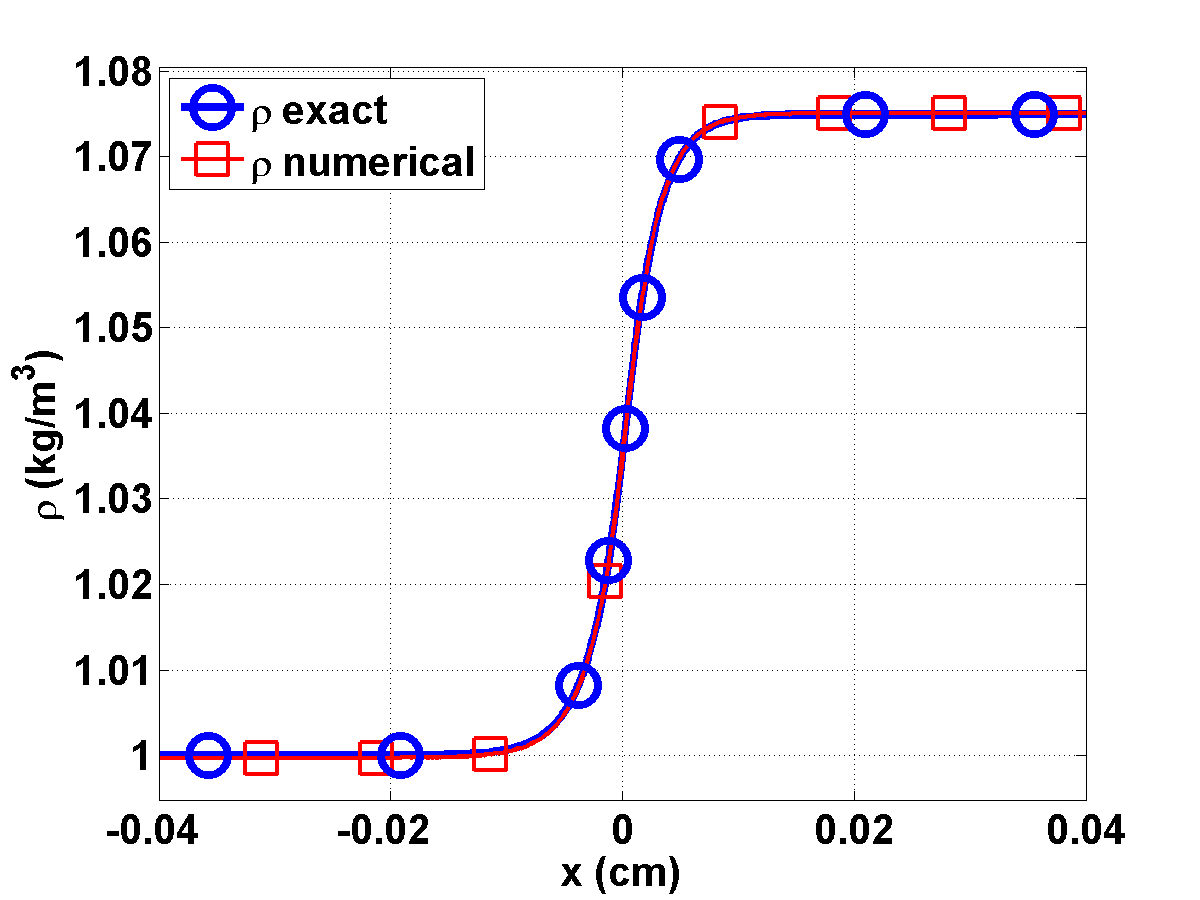
\includegraphics[width=\textwidth]{figures/Mach_1p05_nel_500_density}
        \caption{Material density profile at steady state for Mach 1.05 test.}\label{fig:Mach105_density}
\end{figure}
\begin{figure}[H]
                \centering
                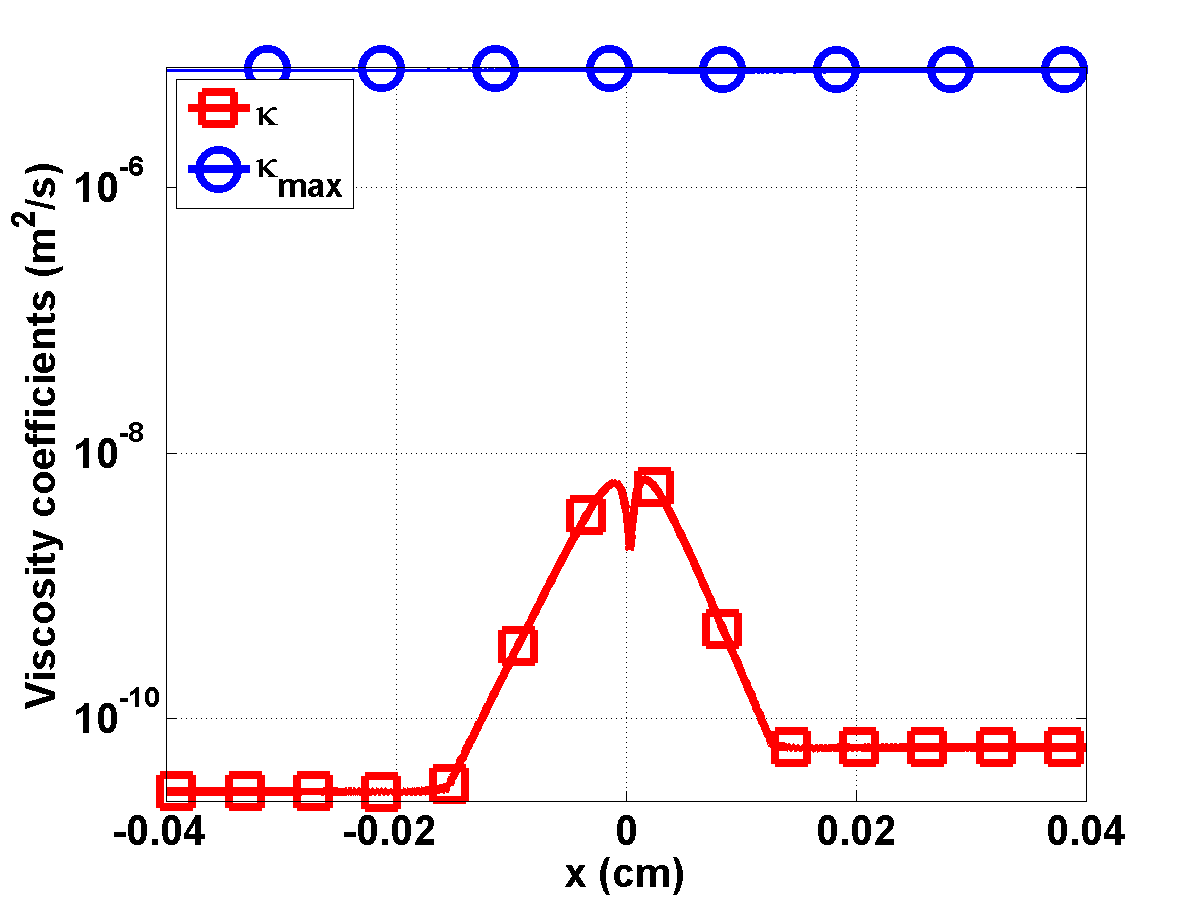
\includegraphics[width=\textwidth]{figures/Mach_1p05_nel_500_viscosity.png}
        \caption{First-order viscosity $\kappa_{max}$ and second-order viscosity $\kappa$ profiles at steady state for Mach 1.05 test (logarithm scale).}\label{fig:Mach105_viscosity}
\end{figure}
The energy transfer between the material and radiation fields is not large enough to form a shock in the material. Thus, all of the material variables are smooth (\fig{fig:Mach105_temp} and \fig{fig:Mach105_density}) as well as the radiation temperature $\theta$. Because of the smoothness of the solution, the viscosity coefficient $\kappa$ is three order of magnitude smaller than the first-order viscosity coefficient $\kappa_{max}$ (\fig{fig:Mach105_viscosity}).

%%%%%%%%%%%%%%%%%%%%%%%%%%%%%%%%%%%%%%%%%%%%%%%%%%%%%%%%%%%%%
\subsubsection{A $1.2$ mach hydrodynamic shock}
%%%%%%%%%%%%%%%%%%%%%%%%%%%%%%%%%%%%%%%%%%%%%%%%%%%%%%%%%%%%%

In this test, the material experiences a shock and the radiation energy density remains smooth. The initial conditions, corresponding to a Mach number of $1.2$ at the inlet, are as follows: 
\begin{table}[H]
\caption{\label{tbl:table4} Initial conditions for mach $1.2$.}
\begin{center}
\begin{tabular}{|c|c|c|}
\hline 
 & left  & right \\ \hline
$\rho$ $(g/cm^3)$ &$1.$ & $1.0749588$ \\ \hline
$u$ $(cm/sh)$& $0.1405588$ & $0.1083456$ \\ \hline
$T$ $(keV)$& $0.1$ & $0.1194751$\\ \hline
$\epsilon$ $(jerks/cm^3)$ & $1.372$ $10^{-6}$ & $2.7955320$ $10^{-6}$\\
\hline
\end{tabular}  
\end{center}  
\end{table}
The slab thickness is set to $L=0.045$ $cm$ and the initial step was located at $x_0 = 0$ $cm$. 
\begin{figure}[H]
       \centering
       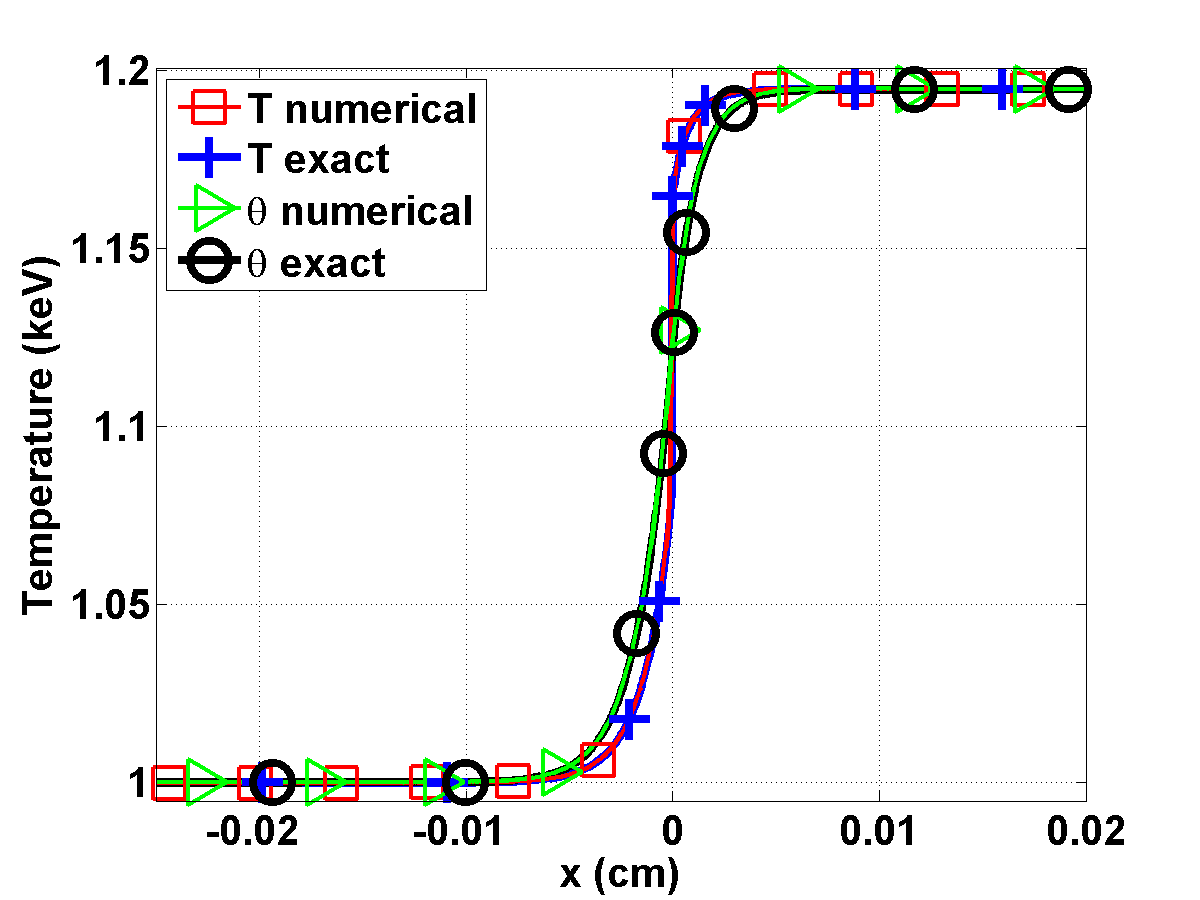
\includegraphics[width=\textwidth]{figures/Mach_1p2_nel_1000_temperature.png}
       \caption{Material and radiation temperature profiles at steady state for Mach 1.2 test.}\label{fig:Mach12_temp}
\end{figure}
The radiation and material temperatures have two different behaviors (\fig{fig:Mach12_temp}): the later experiences an embedded hydrodynamic shock, whereas the radiation temperature is smooth because of the diffusion term. The material temperature profile does not show any pre- and post-shock oscillations. In \fig{fig:Mach12_density}, the material density profile has a shock as well. The viscosity coefficient (\fig{fig:Mach12_viscosity}) is peaked in the shock as expected but does not saturate to the first-order viscosity. It is conjectured that the diffusion term in the radiation equation brings extra stability to the system. \\
Overall, the numerical solution behaves as expected in the shock and the entropy-based viscosity method seems to efficiently stabilize the numerical scheme.  
\begin{figure}[H]
                \centering
                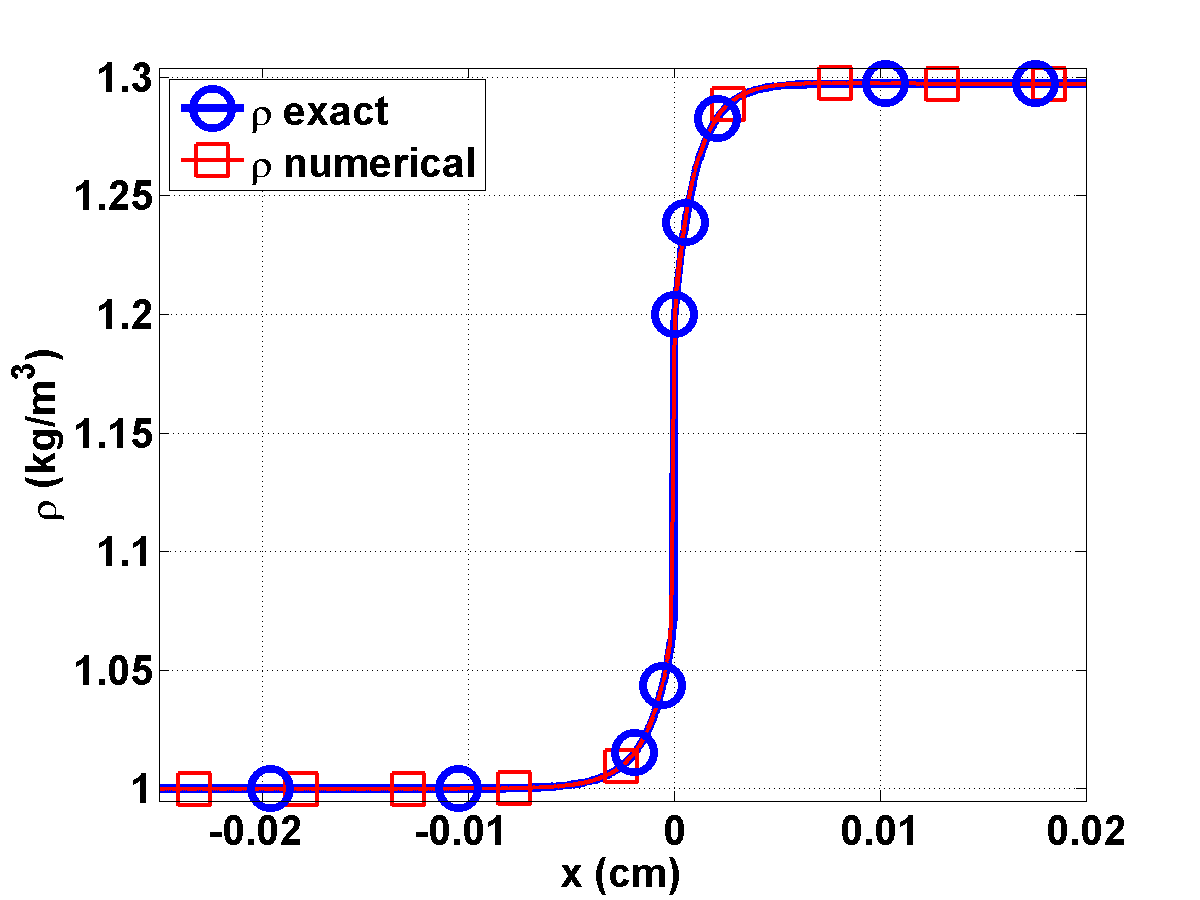
\includegraphics[width=\textwidth]{figures/Mach_1p2_nel_1000_density.png}
        \caption{Material density profile at steady state for Mach 1.2 test.}\label{fig:Mach12_density}
\end{figure}
\begin{figure}[H]
                \centering
                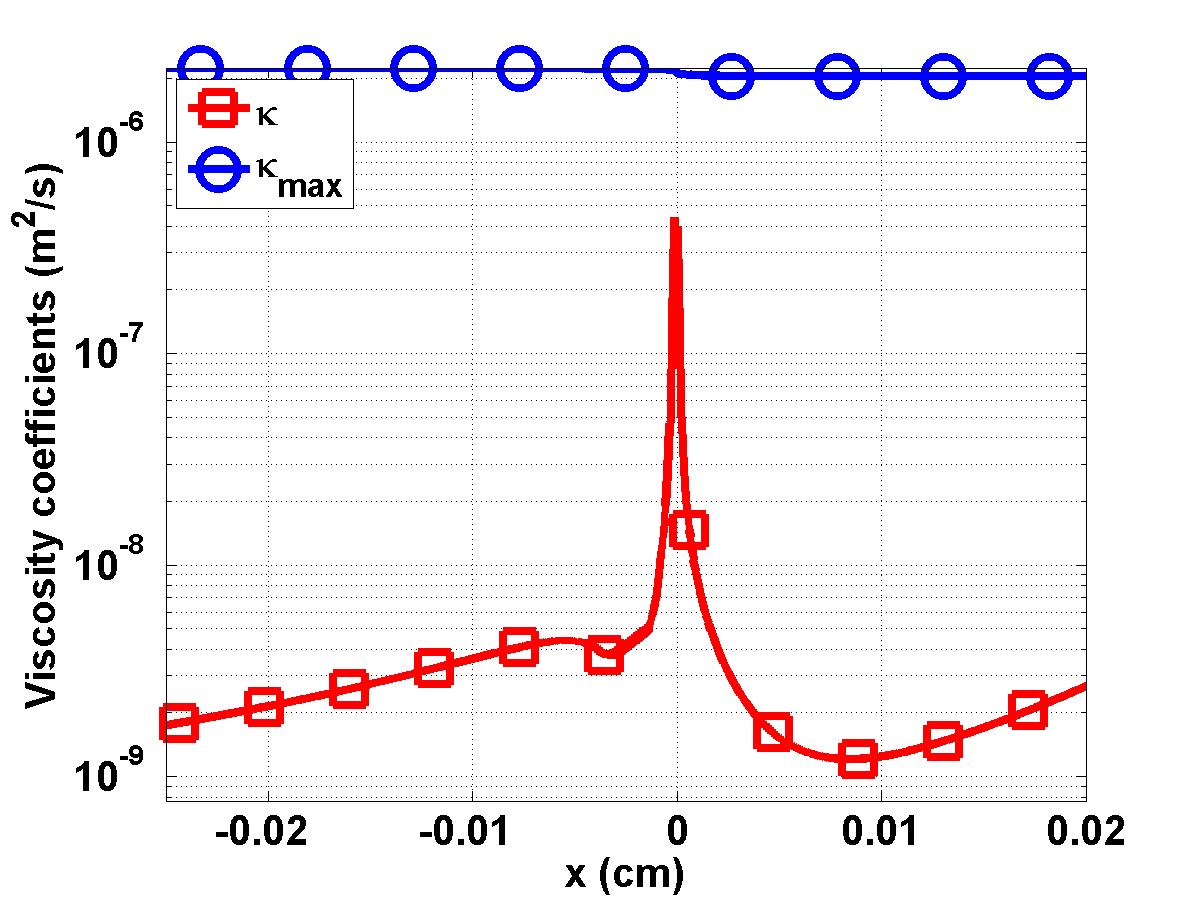
\includegraphics[width=\textwidth]{figures/Mach_1p2_nel_1000_viscosity.png}
        \caption{First-order viscosity $\kappa_{max}$ and second-order viscosity $\kappa$ profiles at steady state for Mach 1.2 test (logarithm scale).}\label{fig:Mach12_viscosity}
\end{figure}

%%%%%%%%%%%%%%%%%%%%%%%%%%%%%%%%%%%%%%%%%%%%%%%%%%%%%%%%%%%%%
\subsubsection{A mach $2$ shock}
%%%%%%%%%%%%%%%%%%%%%%%%%%%%%%%%%%%%%%%%%%%%%%%%%%%%%%%%%%%%%

The Mach $2$ shock test has two features: a hydrodynamic shock and a Zeldovich spike, which make it interesting for testing the robustness of the entropy-based viscosity method. The initial conditions are specified in \tbl{tbl:table5} for a slab of length $L=0.04$ $cm$ with $x_0 = 0.$ $cm$.
\begin{table}[H]
\caption{\label{tbl:table5} Initial conditions for mach $2$.}
\begin{center}
\begin{tabular}{|c|c|c|}
\hline 
 & left  & right \\ \hline
$\rho$ $(g/cm^3)$ &$1.$ & $1.0749588$ \\ \hline
$u$ $(cm/sh)$& $0.1405588$ & $0.1083456$ \\ \hline
$T$ $(keV)$& $0.1$ & $0.1194751$\\ \hline
$\epsilon$ $(jerks/cm^3)$ & $1.372$ $10^{-6}$ & $2.7955320$ $10^{-6}$\\
\hline
\end{tabular}  
\end{center}  
\end{table}
\begin{figure}[H]
                \centering
                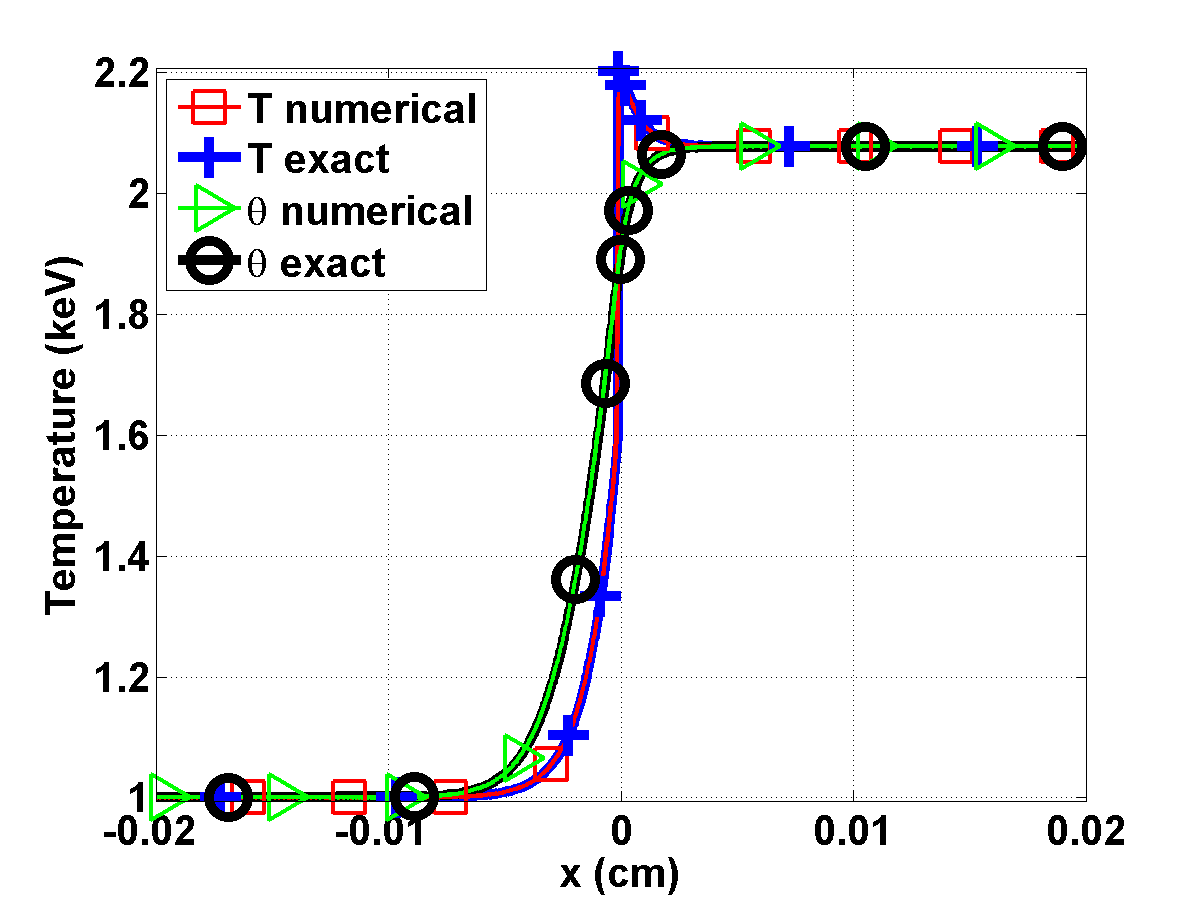
\includegraphics[width=\textwidth]{figures/Mach_2_nel_2000_temperature.png}
        \caption{Material and radiation temperature profiles at steady state for Mach 2 test.}\label{fig:Mach2_temp}
\end{figure}
Once again, the radiation temperature profile is smooth and the material temperature experiences an embedded hydrodynamic shock and a peak as shown in \fig{fig:Mach2_temp}. In \fig{fig:Mach2_density}, the shock is well resolved. The viscosity coefficient profile is given in \fig{fig:Mach2_viscosity} and is peaked, once again, in the shock region. 

For comparison purpose, the same simulation was run with the first-order viscosity only, i.e., $\kappa$ was set equal to $\kappa_{max}$ for the whole domain in order to see the advantage of using a second-order viscosity coefficient. The results are given in \fig{fig:Mach2_tempEVandFO} for the material density and temperature. Numerical solutions with first- and second-order viscosity coefficients are graphed. The radiation temperature profile (not shown here) is not affected much by the first-order viscosity and the curves are coincident. This is expected because of the way the artificial viscosity term is treated in the radiation equation (\sect{sec:entropy-visc-meth_sct5}). However, on the same figure, the shock and peak in the material temperature profile are smoothed out: the shock is not as sharp and the peak amplitude is reduced because of the larger amount of viscosity added to the system. This test shows the benefits of using a high-order viscosity coefficient in order to avoid over-dissipation.
\begin{figure}[H]
                \centering
                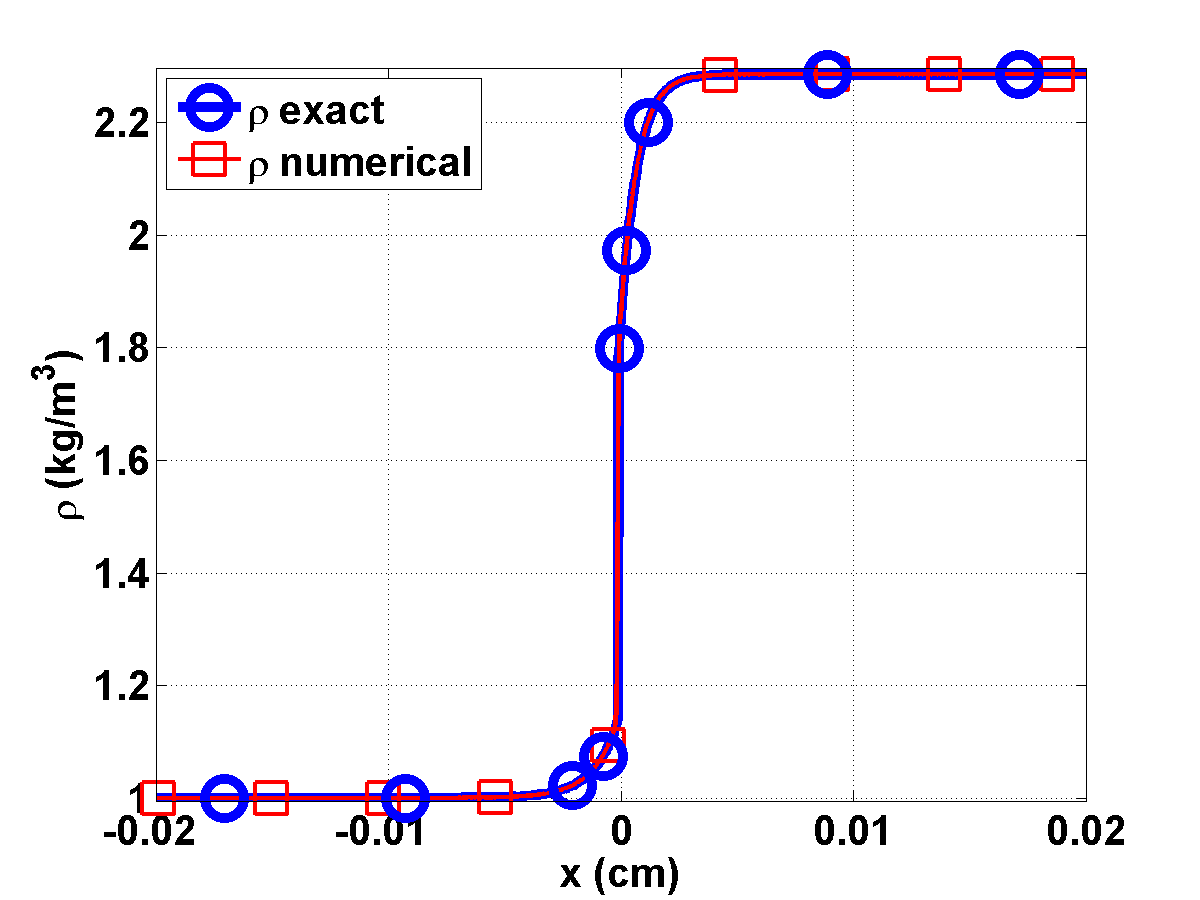
\includegraphics[width=\textwidth]{figures/Mach_2_nel_2000_density.png}
        \caption{Material density profile at steady state for Mach 2 test.}\label{fig:Mach2_density}
\end{figure}
\begin{figure}[H]
                \centering
                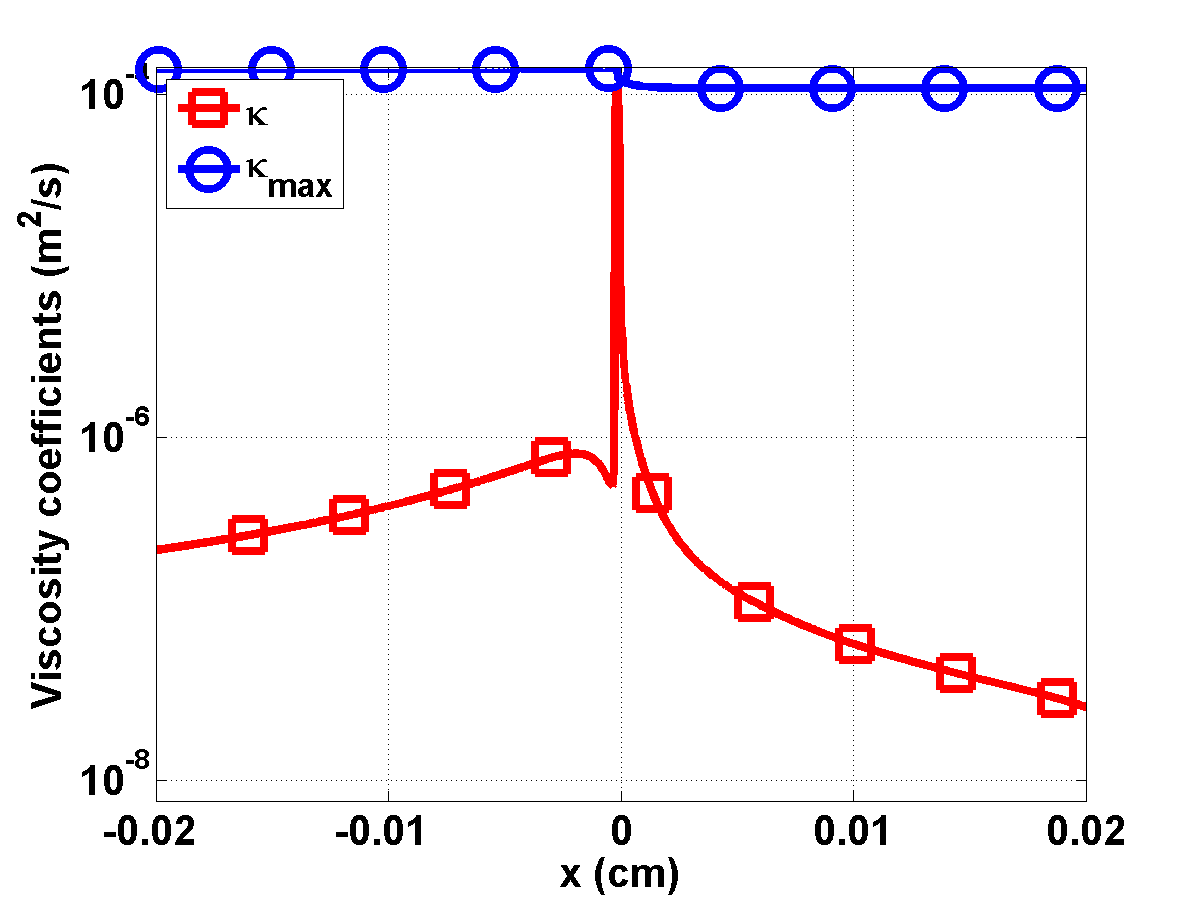
\includegraphics[width=\textwidth]{figures/Mach_2_nel_2000_viscosity.png}
        \caption{First-order viscosity $\kappa_{max}$ and second-order viscosity $\kappa$ profiles at steady state for Mach 2 test.}\label{fig:Mach2_viscosity}
\end{figure}
\begin{figure}[H]
                \centering
                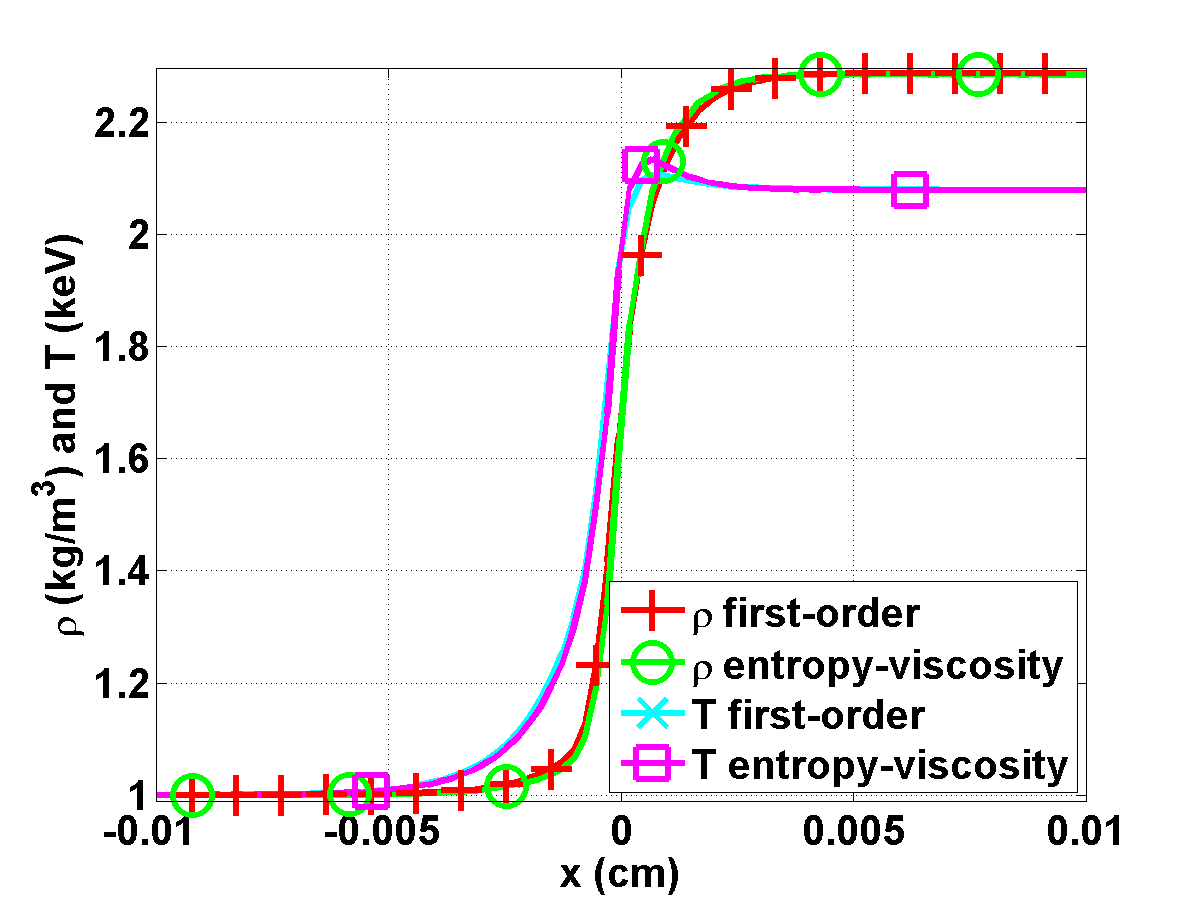
\includegraphics[width=\textwidth]{figures/Mach_2_fo_ev.png}
        \caption{Comprarison between the material density and temperature profiles run with the high-order and first-order viscosity coefficients.}\label{fig:Mach2_tempEVandFO}
\end{figure}

%%%%%%%%%%%%%%%%%%%%%%%%%%%%%%%%%%%%%%%%%%%%%%%%%%%%%%%%%%%%%
\subsubsection{mach $5$ shock}
%%%%%%%%%%%%%%%%%%%%%%%%%%%%%%%%%%%%%%%%%%%%%%%%%%%%%%%%%%%%%

A Mach $5$ test is run with the initial conditions of \tbl{tbl:table6} on a computational domain of length $L=0.05$ $cm$ ($x_0 = 0$ $cm$). Steady-state results are shown in \fig{fig:Mach5_temp}, \fig{fig:Mach5_density}, and \fig{fig:Mach5_viscosity} for the material and radiation temperatures, the density and the viscosity coefficients, respectively.
\begin{table}[H]
\caption{\label{tbl:table6} Initial conditions for mach $5$.}
\begin{center}
\begin{tabular}{|c|c|c|}
\hline 
 & left  & right \\ \hline
$\rho$ $(g/cm^3)$ &$1.$ & $1.0749588$ \\ \hline
$u$ $(cm/sh)$& $0.1405588$ & $0.1083456$ \\ \hline
$T$ $(keV)$& $0.1$ & $0.1194751$\\ \hline
$\epsilon$ $(jerks/cm^3)$ & $1.372$ $10^{-6}$ & $2.7955320$ $10^{-6}$\\
\hline
\end{tabular}  
\end{center}  
\end{table}
\begin{figure}[H]
                \centering
                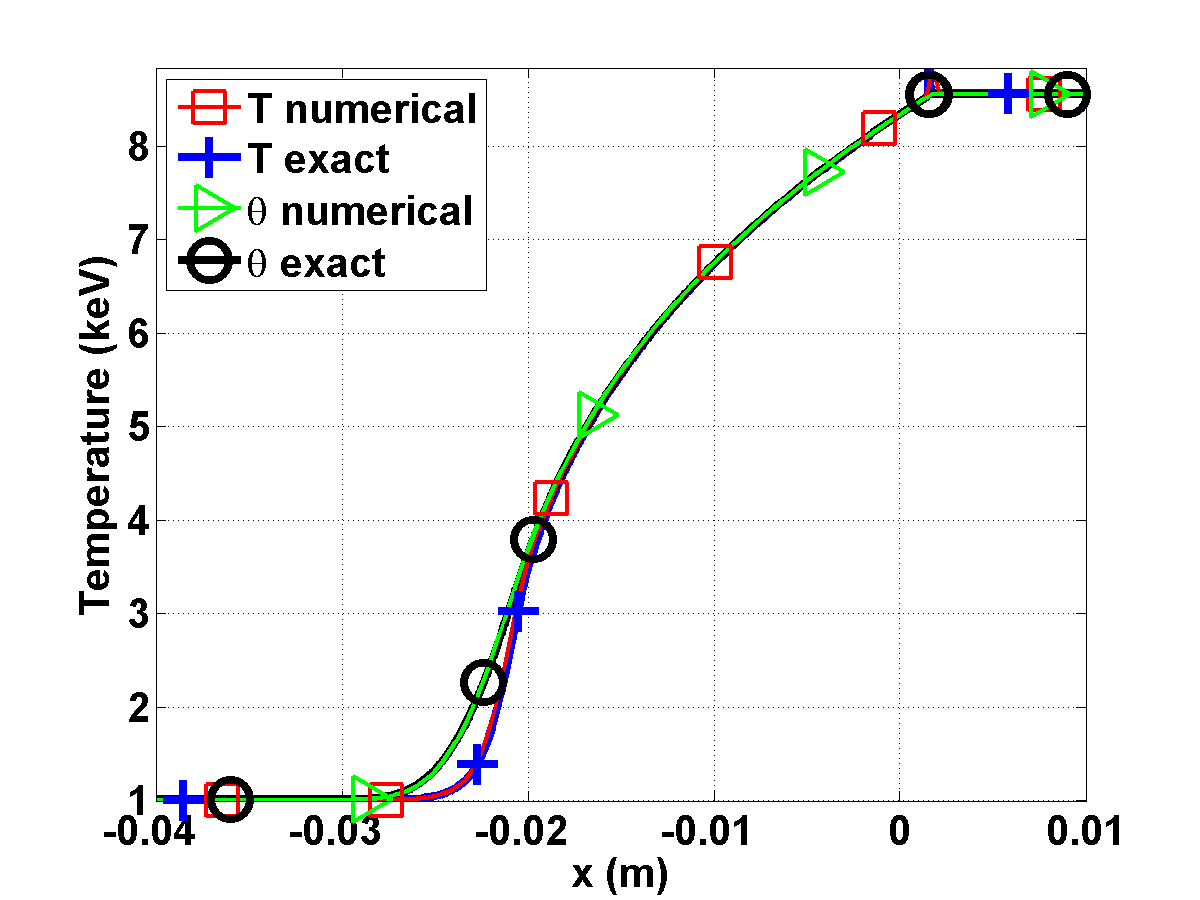
\includegraphics[width=\textwidth]{figures/Mach_5_nel_1000_temperature.png}
        \caption{Material and radiation temperature profiles at steady state for Mach 5 test. Zoom at the location of Zeldovich's spike using different mesh resolutions.}\label{fig:Mach5_temp}
\end{figure}
\begin{figure}[H]
                \centering
                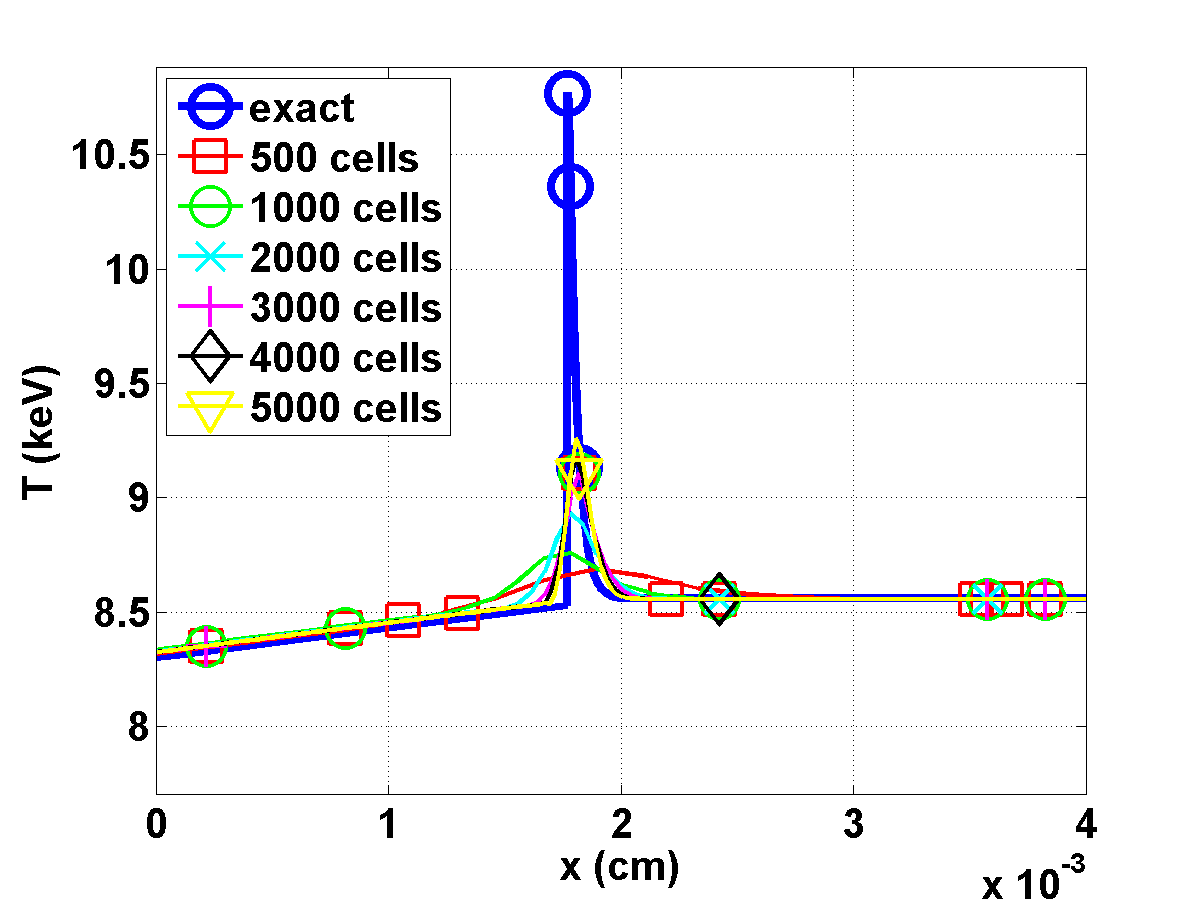
\includegraphics[width=\textwidth]{figures/Mach_5_comparison.png}
        \caption{Material temperature profiles at steady state for the Mach 5 test in the neighborhood spike.}\label{fig:Mach5_comparison}
\end{figure}
In \fig{fig:Mach5_temp}, the radiation temperature profile is smooth. The material temperature no longer exhibits an embedded hydrodynamic shock but shows a Zeldovich spike. The mesh with $500$ elements is not fine enough to correctly resolve the Zeldovich spike. In \fig{fig:Mach5_comparison}, the Zeldovich spike region is plotted for different mesh resolutions, using from $500$ to $5000$ elements: the peak is better resolved when using large numbers of elements and its position seems to be independent of the mesh size when appropriately refined. The density profile, \fig{fig:Mach5_density}, shows a shock located at the same position as the Zeldovich spike of the material temperature profile. The viscosity coefficient $\kappa$ is also peaked in the shock region, as expected. The material and radiation variables do not present any numerical oscillations. 
\begin{figure}[H]
                \centering
                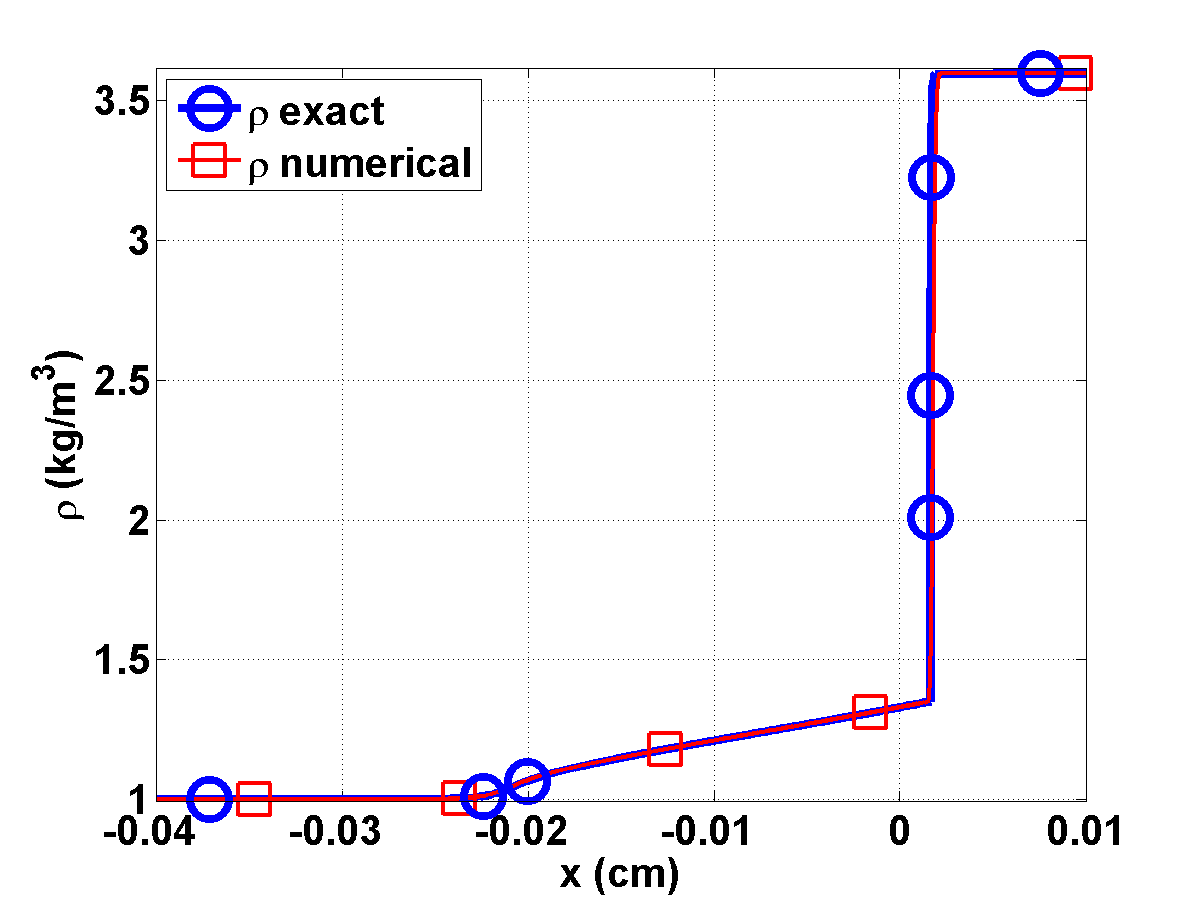
\includegraphics[width=\textwidth]{figures/Mach_5_nel_2000_density.png}
        \caption{Material density profile at steady state for Mach 5 test.}\label{fig:Mach5_density}
\end{figure}
\begin{figure}[H]
                \centering
                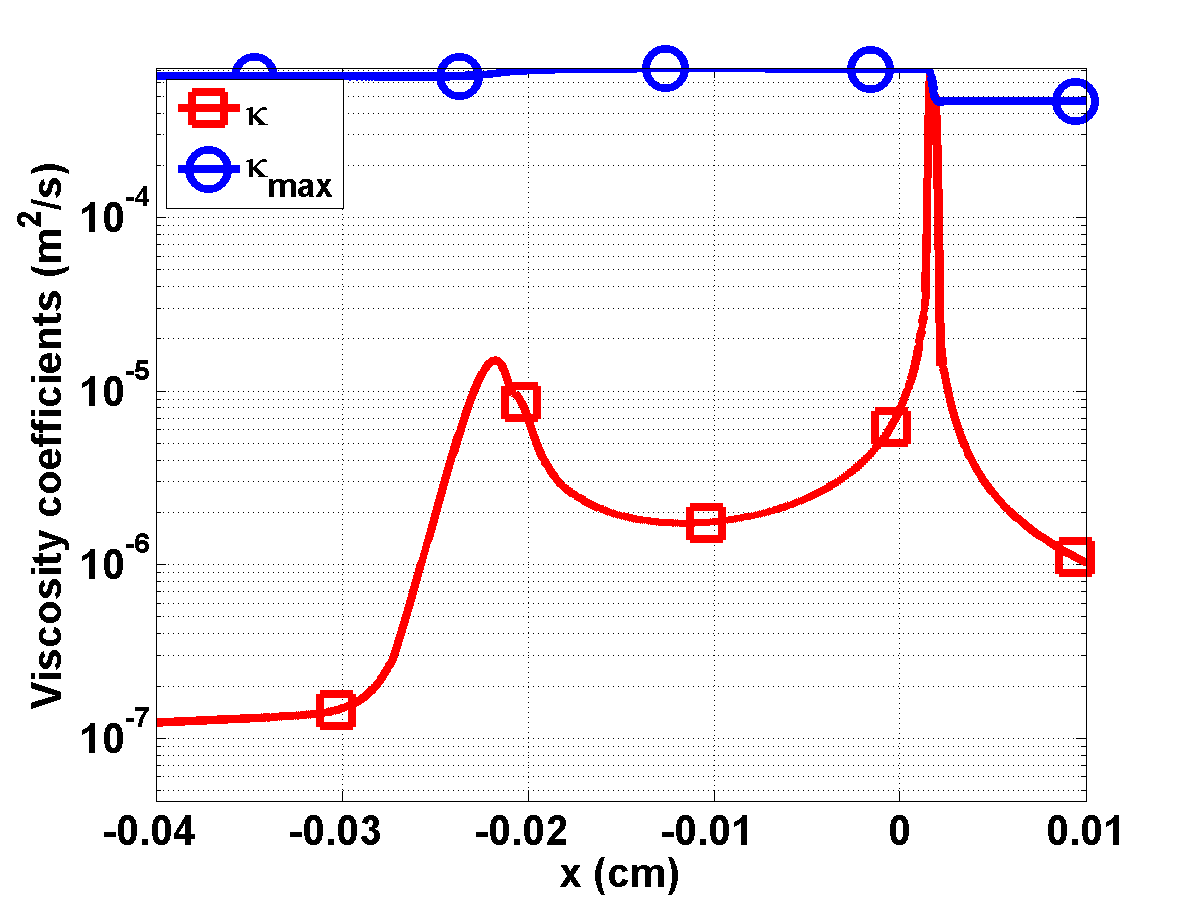
\includegraphics[width=\textwidth]{figures/Mach_5_nel_2000_viscosity.png}
        \caption{First-order viscosity $\kappa_{max}$ and second-order viscosity $\kappa$ profiles at steady state for Mach 5 test.}\label{fig:Mach5_viscosity}
\end{figure}

%%%%%%%%%%%%%%%%%%%%%%%%%%%%%%%%%%%%%%%%%%%%%%%%%%%%%%%%%%%%%
\subsubsection{mach $50$ shock} 
%%%%%%%%%%%%%%%%%%%%%%%%%%%%%%%%%%%%%%%%%%%%%%%%%%%%%%%%%%%%%

The Mach $50$ test is known to be challenging. The initial conditions are given in \tbl{tbl:table7}. The computational domain is of length $L=0.2$ $cm$. Results are once again given at steady state.
\begin{table}[H]
\caption{\label{tbl:table7} Initial conditions for mach $50$.}
\begin{center}
\begin{tabular}{|c|c|c|}
\hline 
 & left  & right \\ \hline
$\rho$ $(g/cm^3)$ &$1.$ & $6.5189217$ \\ \hline
$u$ $(cm/sh)$& $585.6620$ & $89.84031$ \\ \hline
$T$ $(keV)$& $1.0$ & $85.51552$\\ \hline
$\epsilon$ $(jerks/cm^3)$ & $1.372$ $10^{-2}$ & $7.33726$ $10^{5}$\\
\hline
\end{tabular}  
\end{center}  
\end{table}
\begin{figure}[H]
                \centering
                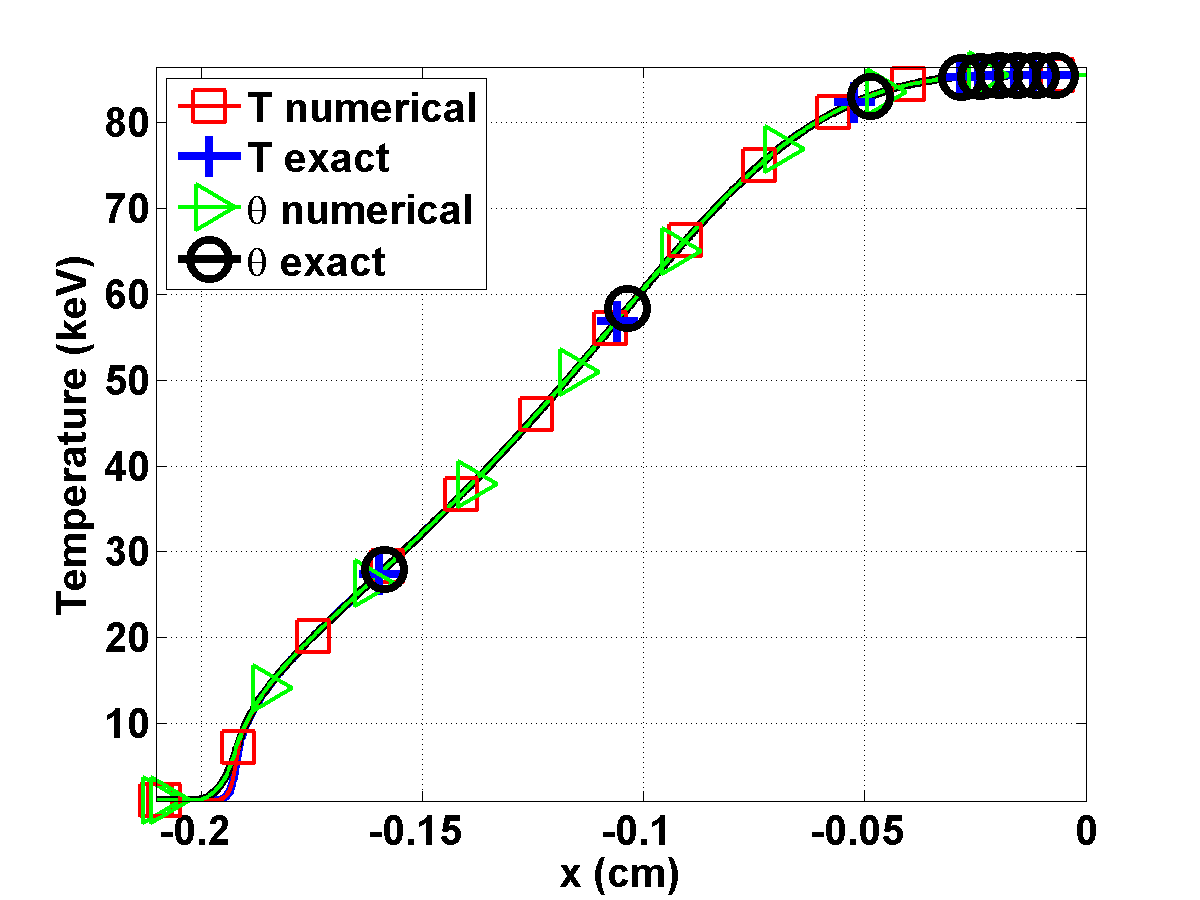
\includegraphics[width=\textwidth]{figures/Mach_50_nel_1000_temperature.png}
        \caption{Material and radiation temperature profiles at steady state for Mach 50 test.}\label{fig:Mach50_temp}
\end{figure}
At Mach $50$, there is no embedded hydrodynamic shock forming as shown in \fig{fig:Mach50_temp}. The density profile is smooth as shown in \fig{fig:Mach50_density}. In \fig{fig:Mach50_temp}, the material and radiation temperatures overlap on all of the computational domain except for a small region located between $x=-0.2$ and $x=-0.18$ $cm$. In this particular region, the viscosity coefficient saturates to the first-order viscosity (see \fig{fig:Mach50_viscosity}) because of the inflection point in the material temperature profile. The artificial dissipative terms correctly stabilize the material temperature profile without altering the physical solution: the radiation temperature is expected to increase ahead of the material temperature.
\begin{figure}[H]
                \centering
                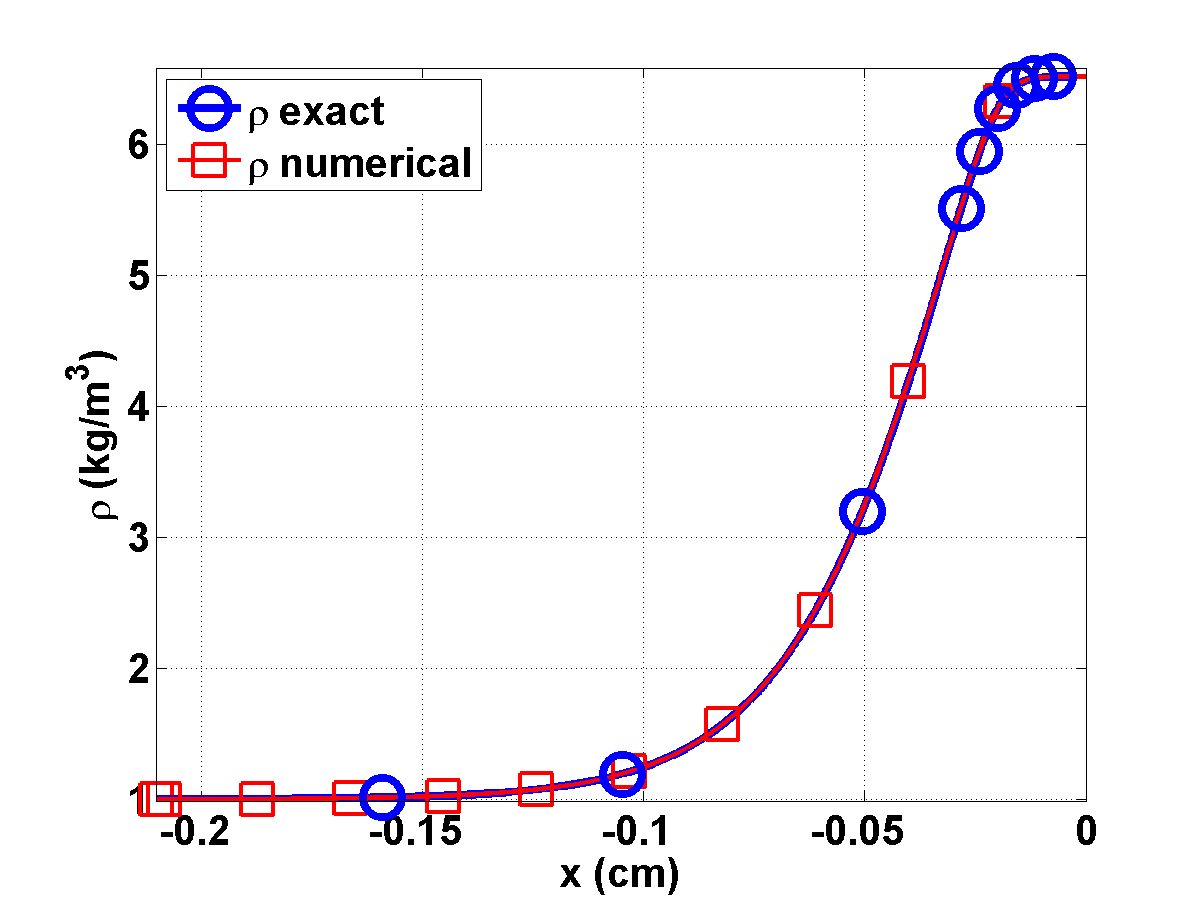
\includegraphics[width=\textwidth]{figures/Mach_50_nel_1000_density.png}
        \caption{Material density profile at steady-state for Mach 50 test.}\label{fig:Mach50_density}
\end{figure}
\begin{figure}[H]
                \centering
                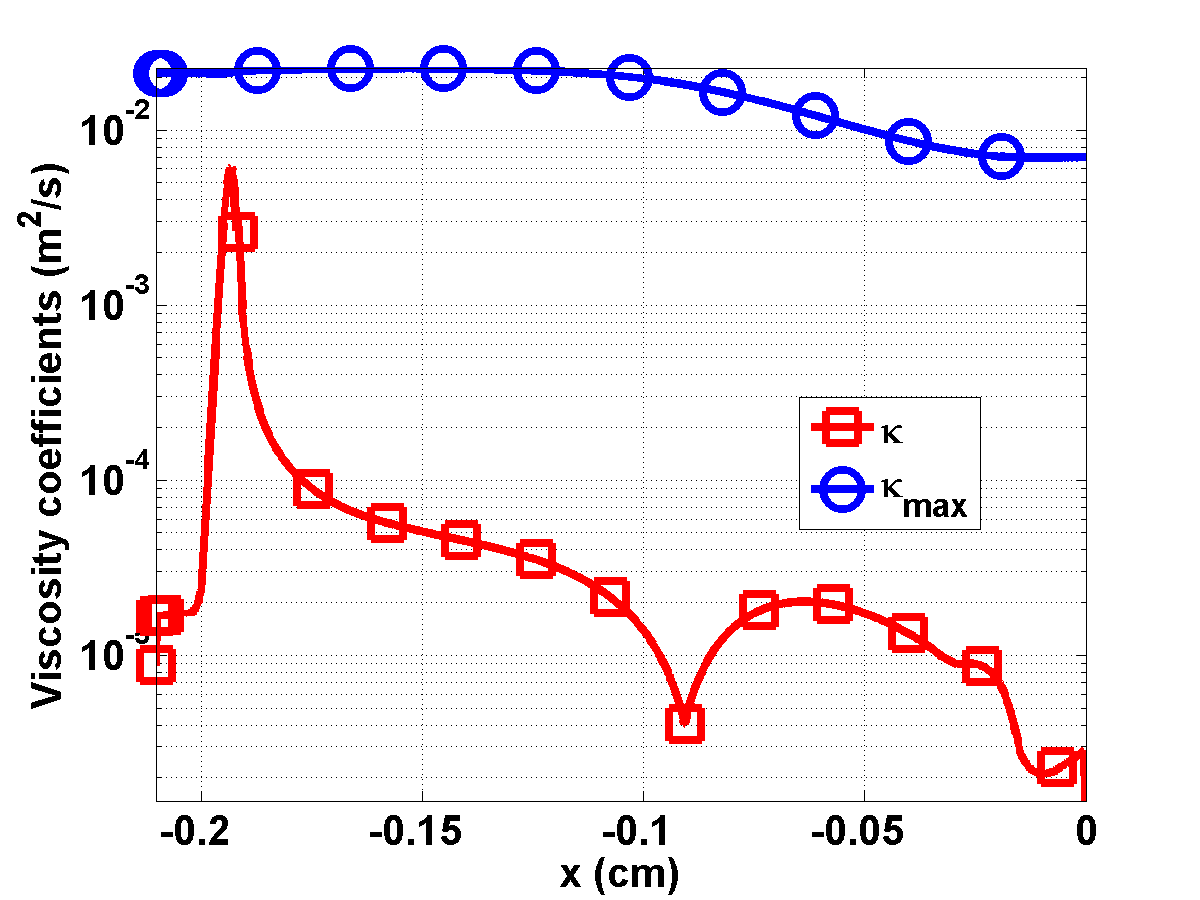
\includegraphics[width=\textwidth]{figures/Mach_50_nel_1000_viscosity.png}
        \caption{First-order viscosity $\kappa_{max}$ and second-order viscosity $\kappa$ profiles at steady-state for Mach 50 test.}\label{fig:Mach50_viscosity}
\end{figure}

%In this chapter, we have shown that the entropy-based viscosity method is a valid candidate for solving the 1-D radiation-hydrodynamic equations. A theoretical derivation is given for the derivation of the dissipative terms that are consistent with the entropy minimum principle. The viscosity coefficient $\kappa$ is defined proportional to the entropy residual that measures the local entropy production allowing detection of shocks. Through the manufactured solution method, it is demonstrated, firstly, that second-order accuracy is achieved when the solution is smooth, and secondly, that the artificial dissipative terms do not affect the physical solution in the equilibrium-diffusion limit. 
%
%The entropy-based numerical scheme also behaves well in the tests performed for Mach numbers ranging from $1.05$ to $50$. The main features such as the embedded hydrodynamic shock and the Zeldovich spike are resolved accurately without spurious oscillations. The viscosity coefficient is peaked in the shock region only and behaves as expected. All of these results were obtained by using an unique definition of the viscosity coefficient that is computed on the fly. The addition of dissipative terms to the set of equations requires more computational work but is rather simple to implement.